\documentclass[12pt, a4paper]{article}

% ── Packages ──────────────────────────────────────────────────────────────────
\usepackage[a4paper, margin=2.5cm]{geometry}
\usepackage{graphicx}
\usepackage{float}
\usepackage{amsmath}
\usepackage{amssymb}
\usepackage{xcolor}
\usepackage{mdframed}
\usepackage{parskip}
\usepackage{enumitem}
\usepackage{titlesec}
\usepackage{booktabs}
\usepackage{hyperref}
\usepackage[T1]{fontenc}
\usepackage[colorinlistoftodos]{todonotes}

% ── Graphics path ─────────────────────────────────────────────────────────────
\graphicspath{{../../Images_for_latex/Lecture_5/}}

% ── Colours ───────────────────────────────────────────────────────────────────
\definecolor{keyblue}{RGB}{30, 80, 160}
\definecolor{keybluebg}{RGB}{220, 235, 255}
\definecolor{noteorange}{RGB}{200, 100, 0}
\definecolor{noteorangebg}{RGB}{255, 240, 215}
\definecolor{warnred}{RGB}{180, 30, 30}
\definecolor{warnredbg}{RGB}{255, 220, 220}
\definecolor{defgreen}{RGB}{20, 110, 50}
\definecolor{defgreenbg}{RGB}{215, 245, 225}
\definecolor{headernavy}{RGB}{25, 35, 90}

% ── Box environments ──────────────────────────────────────────────────────────

% Key Takeaway box (blue)
\newmdenv[
  linecolor=keyblue,
  backgroundcolor=keybluebg,
  linewidth=1.5pt,
  leftline=true, rightline=false, topline=false, bottomline=false,
  innerleftmargin=10pt,
  innerrightmargin=8pt,
  innertopmargin=6pt,
  innerbottommargin=6pt,
  skipabove=8pt,
  skipbelow=8pt,
]{keybox}

% Note box (orange)
\newmdenv[
  linecolor=noteorange,
  backgroundcolor=noteorangebg,
  linewidth=1.5pt,
  leftline=true, rightline=false, topline=false, bottomline=false,
  innerleftmargin=10pt,
  innerrightmargin=8pt,
  innertopmargin=6pt,
  innerbottommargin=6pt,
  skipabove=8pt,
  skipbelow=8pt,
]{notebox}

% Warning box (red)
\newmdenv[
  linecolor=warnred,
  backgroundcolor=warnredbg,
  linewidth=1.5pt,
  leftline=true, rightline=false, topline=false, bottomline=false,
  innerleftmargin=10pt,
  innerrightmargin=8pt,
  innertopmargin=6pt,
  innerbottommargin=6pt,
  skipabove=8pt,
  skipbelow=8pt,
]{warnbox}

% Definition box (green)
\newmdenv[
  linecolor=defgreen,
  backgroundcolor=defgreenbg,
  linewidth=1.5pt,
  leftline=true, rightline=false, topline=false, bottomline=false,
  innerleftmargin=10pt,
  innerrightmargin=8pt,
  innertopmargin=6pt,
  innerbottommargin=6pt,
  skipabove=8pt,
  skipbelow=8pt,
]{defbox}

% ── Section formatting ────────────────────────────────────────────────────────
\titleformat{\section}[block]
  {\large\bfseries\color{headernavy}}
  {}
  {0pt}
  {}
  [\vspace{2pt}\rule{\linewidth}{0.8pt}\vspace{4pt}]

\titleformat{\subsection}[block]
  {\normalsize\bfseries\color{keyblue}}
  {}
  {0pt}
  {}

% ── Commands for inline labels ─────────────────────────────────────────────────
\newcommand{\keynote}[1]{\textbf{\color{keyblue}#1}}
\newcommand{\warn}[1]{\textbf{\color{warnred}#1}}

% ── Document ──────────────────────────────────────────────────────────────────
\begin{document}
\listoftodos
\clearpage

% ── Title ─────────────────────────────────────────────────────────────────────
\begin{center}
  {\LARGE\bfseries\color{headernavy} Sensors \& Systems}\\[4pt]
  {\large Inertial Measurement Units --- Slides 1--8}\\[2pt]
  {\normalsize Jan Bendtsen, Torben Knudsen \quad|\quad Electronic Systems, 8th Semester}
\end{center}

\vspace{4pt}
\hrule height 1.2pt
\vspace{12pt}

% ==============================================================================
%  SECTION 1: Introduction & Overview
% ==============================================================================
\section*{Slides 1--2 \quad Introduction \& Overview}

This lecture introduces \textbf{Inertial Measurement Units (IMUs)} ---
what they are physically, how the individual sensing elements work,
what sources of error affect them, and how a Kalman filter can estimate
both the motion state and the sensor bias simultaneously.

The lecture is structured as follows:

\begin{itemize}[leftmargin=1.4em]
  \item \textbf{Slides 3--8:} What an IMU is, where it is used, and why
        MEMS technology made it ubiquitous.
  \item \textbf{Slides 9--15:} Physical measurement principles ---
        how accelerometers and gyroscopes actually work.
  \item \textbf{Slides 16--21:} The full mathematical measurement model
        and every error source (bias, distortion, noise, temperature\ldots).
  \item \textbf{Slides 22--27:} Simplified models and a Kalman filter that
        estimates position, velocity, acceleration \emph{and} bias at once.
  \item \textbf{Slides 28--33:} Calibration procedures, attitude estimation,
        and sensor fusion filters.
\end{itemize}

% ==============================================================================
%  SECTION 2: What is an IMU?
% ==============================================================================
\clearpage
\section*{Slides 3--4 \quad What Is an IMU?}

\begin{figure}[H]
  \centering
  
\includegraphics[width=0.7\linewidth]{slide-03.jpg}
  \caption{A variety of inertial sensors --- from single-axis MEMS chips
           to complete IMU modules.}
  \label{fig:slide03}
\end{figure}

\subsection*{What does ``inertial'' mean?}

The word \textbf{inertial} means the sensor is \emph{self-contained} ---
it needs no external signal, satellite, or reference point to produce
a measurement. It only reacts to forces and rotations acting on the
body it is attached to.

This is the key distinction from sensors that rely on something external:

\begin{center}
\renewcommand{\arraystretch}{1.5}
\begin{tabular}{lll}
  \toprule
  \textbf{Sensor} & \textbf{What it measures} & \textbf{Needs external signal?} \\
  \midrule
  IMU (accelerometer + gyro) & Forces \& rotation on the body & No --- fully self-contained \\
  GNSS / GPS                 & Absolute position on Earth      & Yes --- satellite signals \\
  Camera                     & Visual features in the scene    & Yes --- ambient light \\
  LiDAR                      & Distance to surrounding objects & Yes --- laser returns \\
  Barometer                  & Atmospheric pressure (altitude) & Partially --- ambient air \\
  Magnetometer               & Earth's magnetic field (heading) & No --- but Earth-referenced \\
  \bottomrule
\end{tabular}
\end{center}

\begin{notebox}
  \textbf{Why does self-containment matter?}\\
  A GNSS receiver loses signal inside buildings, tunnels, and underwater.
  A camera fails in darkness or heavy fog.
  LiDAR becomes expensive and bulky.
  The IMU works in all of these environments because it only measures
  what the body itself is doing --- not anything in the outside world.\\[4pt]
  The trade-off is \textbf{drift}: because an IMU never sees an absolute
  reference, small measurement errors accumulate over time.
  That is why IMUs are almost always \emph{fused} with a slower
  absolute sensor (GNSS, camera) that corrects the growing error.
\end{notebox}

\subsection*{The three sensor types inside an IMU}

\begin{defbox}
  \textbf{Inertial Measurement Unit (IMU)}\\
  An IMU combines three sensor types, each measuring along three
  orthogonal axes ($x$, $y$, $z$), giving nine total measurement
  channels:

  \begin{itemize}[leftmargin=1.4em, topsep=4pt]
    \item \textbf{Accelerometer} --- measures \emph{specific force}:
          the total force per unit mass acting on the proof mass,
          which includes both actual linear acceleration \emph{and}
          gravity. Unit: m/s$^2$.\\
          \textit{Example:} Sitting flat on a desk the accelerometer
          reads $+9.81$\,m/s$^2$ upward (the desk pushes the mass up).
          In free-fall it reads $0$ --- because there is no contact
          force at all.

    \item \textbf{Gyroscope} --- measures \emph{angular velocity}:
          how fast the body is rotating around each axis. Unit: rad/s
          (or °/s).\\
          \textit{Example:} Turning your head to the right at a steady
          speed of roughly $1$\,rad/s, the gyroscope $z$-axis
          (yaw) reads $+1$\,rad/s.

    \item \textbf{Magnetometer} --- measures the local magnetic field
          vector. Unit: $\mu$T (microtesla).\\
          \textit{Example:} Like a 3-D compass --- it tells you the
          direction of Earth's magnetic north in the body frame, so
          you can compute heading (yaw) even without GPS.
          It is affected by nearby metal objects and electronics.
  \end{itemize}
\end{defbox}

% ── Slide 4 ───────────────────────────────────────────────────────────────────
\subsection*{Slide 4 --- Key numbers and their meaning}

\begin{figure}[H]
  \centering
  
\includegraphics[width=\linewidth]{slide-04.jpg}
  \caption{A compact consumer IMU module. All nine channels are on a
           single chip a few millimetres across, sampled at up to
           1000\,Hz.}
  \label{fig:slide04}
\end{figure}

The slide's four bullet points in plain terms:

\begin{center}
\renewcommand{\arraystretch}{1.5}
\begin{tabular}{p{5.2cm} p{8.5cm}}
  \toprule
  \textbf{Slide value} & \textbf{What it means} \\
  \midrule
  100\,Hz to 1000\,Hz &
    New IMU reading every 1--10\,ms.
    A camera gives one frame every 33\,ms (30\,Hz).
    The IMU is \textbf{10--100$\times$ faster}. \\
  Faster than cameras, LiDARs, depth sensors &
    Those sensors run at 10--60\,Hz --- far too slow to stabilise
    fast dynamics like a drone or rocket in real time. \\
  Primary tool for short-term state estimation &
    Over a fraction of a second the IMU is very accurate.
    Over minutes, small errors add up and the position drifts
    (see bias example below). \\
  Essential for process updates in Kalman filters &
    The IMU feeds the \emph{prediction step} of the Kalman filter
    at full speed --- keeping the state estimate fresh between
    slow GPS or camera corrections. \\
  \bottomrule
\end{tabular}
\end{center}

\textbf{Why short-term only? --- the drift problem.}
When you integrate an accelerometer reading to get velocity,
and integrate again to get position, any small constant error
(bias) gets amplified:
a bias of just $0.01$\,m/s$^2$ gives a velocity error of
$0.6$\,m/s and a position error of \textbf{18\,m} after
only one minute.
The IMU is trusted for short windows; an external sensor
(GPS, camera) must correct it regularly.
\todo{Go Back and Look at this drift problem}
\subsection*{The Kalman filter prediction and update steps}

\begin{notebox}
  \textbf{What the two Kalman steps actually do:}\\[4pt]
  \textbf{Prediction step} (runs at IMU rate, e.g.\ 500\,Hz)\\
  \textit{Input:} new IMU reading --- acceleration $a_k$ and
  angular rate $\omega_k$.\\
  \textit{What happens:} the filter uses the dynamics model to
  roll the current state estimate forward by one time step $T_s$.\\
  \textit{Output:} a \emph{predicted} state estimate
  $\hat{x}_{k+1|k}$ --- position, velocity, orientation ---
  valid right now, but slightly uncertain because the model
  is not perfect and IMU noise adds up.\\[6pt]
  %
  \textbf{Update step} (runs only when a new external measurement arrives)\\
  \textit{Input:} new measurement from GPS, camera, or another
  slow sensor (e.g.\ GPS position fix every 200\,ms).\\
  \textit{What happens:} the filter compares the new measurement
  to what it \emph{predicted} it would see, and nudges the
  state estimate toward the truth by an amount controlled by
  the Kalman gain $K_k$.\\
  \textit{Output:} a \emph{corrected} state estimate
  $\hat{x}_{k|k}$ --- this is the final answer the system uses:
  estimated position, velocity, orientation, and even estimated
  bias.\\[6pt]
  %
  The update step does \textbf{not} simply replace the old estimate
  with the sensor reading --- it \emph{blends} the two based on
  how much it trusts each one (sensor noise $R$ vs.\ prediction
  uncertainty $P$).
\end{notebox}

\begin{notebox}
  \textbf{Concrete timing example:}\\
  GPS at 5\,Hz (new fix every 200\,ms).
  IMU at 500\,Hz (new reading every 2\,ms).\\
  In each 200\,ms gap: \textbf{100 prediction steps} (IMU-driven,
  state kept up to date) then \textbf{1 update step} (GPS-driven,
  drift corrected).\\
  The output of the system after each update step is a smoothly
  running estimate of position, velocity and orientation ---
  updated at 500\,Hz, corrected at 5\,Hz.
\end{notebox}

\begin{keybox}
  \textbf{Key takeaways --- Slides 3--4}
  \begin{itemize}[leftmargin=1.4em, topsep=2pt]
    \item \textbf{Inertial} = self-contained; no satellite, light, or
          external signal needed --- works indoors, underwater, and
          in darkness.
    \item Three sensor types: accelerometer (force/gravity),
          gyroscope (angular rate), magnetometer (magnetic heading).
    \item 100--1000\,Hz = new data every 1--10\,ms,
          far faster than cameras (30\,Hz) or LiDAR (10--20\,Hz).
    \item Short-term accurate, long-term drifty ---
          always fused with a slower absolute sensor (GNSS, camera)
          that corrects the accumulated error.
    \item In a Kalman filter: IMU = prediction step (fast),
          external sensor = update step (slow).
  \end{itemize}
\end{keybox}

% ==============================================================================
%  SECTION 3: Applications & Need for Calibration
% ==============================================================================
\section*{Slides 5--6 \quad Applications \& Need for Calibration}

\begin{figure}[H]
  \centering
  
\includegraphics[width=0.80\linewidth]{slide-05.jpg}
  \caption{IMUs are used wherever fast orientation and motion data
           are needed.}
  \label{fig:slide05}
\end{figure}

\subsection*{Applications}

IMUs appear in almost every system that needs real-time orientation
or motion information:

\begin{itemize}[leftmargin=1.4em]
  \item \textbf{Aerial and underwater robotics} --- drones and AUVs use
        IMUs for attitude control and navigation.
  \item \textbf{Ground vehicles and rockets} --- self-navigating cars,
        missiles, and launch vehicles rely on inertial navigation to
        operate in GPS-denied environments.
  \item \textbf{Consumer electronics} --- VR/AR headsets (e.g.\ Oculus),
        game controllers (Nintendo Wii remote), and smartphones all
        contain MEMS IMUs.
  \item \textbf{Aviation} --- Inertial Navigation Systems (INS) fuse
        IMU data over long flights to keep the aircraft on track
        between GPS fixes.
\end{itemize}

\begin{figure}[H]
  \centering
  
\includegraphics[width=0.80\linewidth]{slide-06.jpg}
  \caption{Raw IMU data without calibration is unreliable ---
           errors compound rapidly.}
  \label{fig:slide06}
\end{figure}

\subsection*{Why calibration is essential}

\begin{notebox}
  Every physical IMU has \textbf{noise} (random fluctuations on every
  reading) and \textbf{bias} (a constant or slowly varying offset even
  when the sensor is perfectly still).
  If you feed raw, uncorrected measurements into a navigation algorithm,
  these errors accumulate: a small constant bias on an accelerometer
  integrates into a velocity error that grows linearly in time, and
  then into a position error that grows quadratically.\\[4pt]
  Calibration builds an accurate \emph{mathematical model} of every
  error source so that the filter can correct for them.
  The rest of this lecture is essentially the story of
  \emph{identifying} those error sources and \emph{modelling} them
  precisely enough to be useful.
\end{notebox}

\begin{keybox}
  \textbf{Key takeaways --- Slides 5--6}
  \begin{itemize}[leftmargin=1.4em, topsep=2pt]
    \item IMUs are everywhere --- from sub-2-EUR MEMS chips in phones
          to high-precision units in aircraft INS.
    \item Raw measurements are always corrupted by noise and bias.
    \item Without calibration, integration of accelerometer data leads
          to rapidly growing position errors.
    \item Calibration = building a model of the errors so a filter
          can undo them.
  \end{itemize}
\end{keybox}

% ==============================================================================
%  SECTION 4: Terminology & MEMS Technology
% ==============================================================================
\section*{Slides 7--8 \quad Terminology \& MEMS Technology}

\begin{figure}[H]
  \centering
  
\includegraphics[width=0.80\linewidth]{slide-07.jpg}
  \caption{Common marketing terminology around IMUs is often technically
           imprecise.}
  \label{fig:slide07}
\end{figure}

\subsection*{Clearing up the terminology}

\begin{warnbox}
  \textbf{``6-axis gyroscope'' is wrong.}\\
  A single gyroscope measures rotation around \emph{one} axis.
  A 3-axis gyroscope chip measures around three axes (roll, pitch, yaw).
  There is no such thing as a 6-axis gyroscope --- what is usually
  meant is a \emph{6-axis IMU}: a 3-axis accelerometer combined with
  a 3-axis gyroscope on one chip.
  The label ``6-axis'' counts the total number of measurement axes,
  not the number of sensors.
\end{warnbox}

\begin{defbox}
  \textbf{Axis count convention}
  \begin{itemize}[leftmargin=1.4em, topsep=2pt]
    \item \textbf{6-axis IMU} --- 3-axis accelerometer + 3-axis gyroscope.
    \item \textbf{9-axis IMU} --- 3-axis accelerometer + 3-axis gyroscope
          + 3-axis magnetometer.
  \end{itemize}
  \vspace{4pt}
  \textbf{Degrees of Freedom (DoF):}\\
  A \emph{degree of freedom} is an independent direction in which
  something can move or rotate.
  A free rigid body in 3-D space has \textbf{6 DoF}:
  \begin{itemize}[leftmargin=1.4em, topsep=2pt]
    \item 3 \textbf{translational} --- move left/right ($x$),
          forward/backward ($y$), up/down ($z$).
    \item 3 \textbf{rotational} --- roll (tilt sideways),
          pitch (tilt forward/back), yaw (turn left/right).
  \end{itemize}
  Think of a drone: it can slide in any of the three directions
  \emph{and} rotate around any of the three axes --- that is 6
  independent ways it can move, hence 6 DoF.\\[4pt]
  The IMU does \emph{not} have its own DoF.
  It is a measuring instrument bolted onto the body.
  What it does is give you the data needed to \emph{estimate}
  which of those 6 directions the body is currently moving or
  rotating in --- it does not itself move freely in 6 directions.
\end{defbox}

\begin{figure}[H]
  \centering
  
\includegraphics[width=0.80\linewidth]{slide-08.jpg}
  \caption{MEMS fabrication --- a spring-mass structure etched directly
           into silicon, with readout electronics on the same chip.}
  \label{fig:slide08}
\end{figure}

\subsection*{What is MEMS?}

\begin{notebox}
  \textbf{Micro-Electro-Mechanical Systems (MEMS)} means a tiny
  mechanical structure --- a spring and a small suspended mass ---
  etched directly into silicon, on the same chip as the readout
  electronics.
  The mass is not rigidly fixed; because of the spring it shifts
  slightly relative to the chip when the device accelerates, and
  that displacement is measured electrically.\\[4pt]
  Because everything is on one chip a few millimetres across,
  MEMS sensors are cheap, small, and low-power.
  The full physics of \emph{how} displacement becomes an acceleration
  measurement is covered in Section~2 (slides 9--15).
\end{notebox}

\begin{keybox}
  \textbf{Key takeaways --- Slides 7--8}
  \begin{itemize}[leftmargin=1.4em, topsep=2pt]
    \item ``6-axis'' = accel + gyro; ``9-axis'' = accel + gyro + mag.
          Never say ``6-axis gyroscope''.
    \item The IMU estimates the body's 6 DoF state; it does not
          \emph{have} DoF.
    \item MEMS technology started with automotive airbag requirements
          and scaled to billions of chips per year.
    \item Mass production means a consumer 9-axis IMU now costs
          2--5\,EUR while incorporating real-time thermal correction.
  \end{itemize}
\end{keybox}

% ==============================================================================
%  SECTION 2: Measurement Principles
% ==============================================================================
\clearpage
\section*{Slides 9--10 \quad MEMS Accelerometer: Principle \& Gravity}

% ── Slide 9 ───────────────────────────────────────────────────────────────────
\subsection*{The mass-spring system}

\begin{figure}[H]
  \centering
  
\includegraphics[width=0.80\linewidth]{slide-09.jpg}
  \caption{A MEMS accelerometer: a proof mass suspended by silicon springs
           inside a sealed cavity on the chip.}
  \label{fig:slide09}
\end{figure}

As promised in Section~1, here is the full physical picture.
A small mass (the \textbf{proof mass}) is suspended by silicon springs
inside the chip.
When the chip accelerates, the mass resists due to inertia, deflecting
the springs by a displacement $z$.
The complete dynamics are described by a second-order differential
equation --- a damped mass-spring system driven by the external force:

\[
  m\ddot{z}(t) + b\dot{z}(t) + kz(t) = F(t)
\]

\begin{center}
\renewcommand{\arraystretch}{1.5}
\begin{tabular}{cll}
  \toprule
  \textbf{Term} & \textbf{Meaning} & \textbf{Role} \\
  \midrule
  $m\ddot{z}$ & Mass $\times$ acceleration of the proof mass
              & Inertia --- resists change \\
  $b\dot{z}$  & Damping coefficient $\times$ velocity
              & Energy loss (air/material friction) \\
  $kz$        & Spring constant $\times$ displacement
              & Restoring force pulling mass back \\
  $F(t)$      & External force applied to the chip body
              & The thing we want to measure \\
  \bottomrule
\end{tabular}
\end{center}

\begin{notebox}
  \textbf{What does the sensor read at steady state?}\\
  Once the acceleration stops changing, the mass stops bouncing and
  sits still at a fixed position relative to the chip.
  ``Still'' means it has zero velocity and zero acceleration of its
  own, so $\ddot{z} = 0$ and $\dot{z} = 0$.
  Plug those into the equation and the inertia and damping terms
  vanish, leaving only the spring:
  \[
    kz_{\text{ss}} = F = ma
    \quad\Longrightarrow\quad
    z_{\text{ss}} = \frac{m}{k}\,a
  \]
  \textbf{What this says in plain words:}
  the spring has stretched just far enough that the spring force
  $kz_{\text{ss}}$ exactly balances the external force $ma$ on the
  mass.
  The mass is not moving anymore --- it is being held in place by
  the spring.\\[4pt]
  The factor $m/k$ is the \textbf{mechanical sensitivity}:
  \begin{itemize}[leftmargin=1.4em, topsep=2pt]
    \item Larger $m$ (heavier mass) $\to$ more inertia $\to$ bigger
          displacement for the same acceleration $\to$ easier to measure,
          but the chip needs more space.
    \item Larger $k$ (stiffer spring) $\to$ spring fights back harder
          $\to$ smaller displacement for the same acceleration $\to$
          harder to measure, but the mass cannot drift too far.
  \end{itemize}
  So $m/k$ is a design trade-off the engineers choose when they
  fabricate the chip.
  Once it is fixed, measuring $z_{\text{ss}}$ and dividing by $m/k$
  directly gives the acceleration $a$.
\end{notebox}

% ── Slide 10 ──────────────────────────────────────────────────────────────────
\subsection*{Gravity vs.\ linear acceleration}

\begin{figure}[H]
  \centering
  
\includegraphics[width=0.80\linewidth]{slide-10.jpg}
  \caption{A stationary sensor tilted under gravity deflects identically
           to one accelerating horizontally --- the two cases are
           indistinguishable from the sensor alone.}
  \label{fig:slide10}
\end{figure}

\begin{warnbox}
  \textbf{The accelerometer cannot tell gravity from motion.}\\
  The spring-mass system responds to \emph{any} force --- it does not
  know whether that force comes from the body accelerating or from
  gravity pulling on the proof mass.\\[4pt]
  Two identical sensor outputs:
  \begin{itemize}[leftmargin=1.4em, topsep=2pt]
    \item A sensor \textbf{lying flat and stationary}: gravity pulls
          the mass downward → spring deflects → reads
          $+9.81$\,m/s$^2$ upward.
    \item A sensor \textbf{accelerating upward at 9.81\,m/s$^2$}:
          inertia pulls the mass downward → spring deflects exactly
          the same way → also reads $+9.81$\,m/s$^2$.
  \end{itemize}
  From the sensor reading alone you \textbf{cannot distinguish} these
  two situations.
  This is actually Einstein's equivalence principle: gravity and
  acceleration are locally indistinguishable.
\end{warnbox}

\begin{notebox}
  \textbf{How this is used and handled:}

  \medskip
  \textbf{Roll and pitch estimation (stationary body):}\\
  Gravity always points straight down in the world --- it never
  changes direction.
  But as you \emph{tilt the sensor}, its own axes ($x$, $y$, $z$)
  rotate with it, so they now point in different directions relative
  to gravity.
  The result is that gravity gets split differently across the three
  axes depending on how much the sensor is tilted.\\[4pt]
  Example --- sensor lying flat (level):
  \[
    \begin{bmatrix} a_x \\ a_y \\ a_z \end{bmatrix}
    = \begin{bmatrix} 0 \\ 0 \\ g \end{bmatrix}
  \]
  The $z$-axis points straight up and carries all of gravity; $x$ and
  $y$ are horizontal and see none of it.\\[4pt]
  Now tilt the sensor sideways by angle $\theta$ (roll around the
  $x$-axis):
  \[
    \begin{bmatrix} a_x \\ a_y \\ a_z \end{bmatrix}
    = \begin{bmatrix} 0 \\ g\sin\theta \\ g\cos\theta \end{bmatrix}
  \]
  The $y$-axis has rotated so it now has a component pointing
  downward --- it picks up part of gravity.
  The more you tilt, the more gravity ``leaks'' from $z$ into $y$.
  From these two readings you can recover the tilt angle directly:
  \[
    \theta = \arctan\!\left(\frac{a_y}{a_z}\right)
  \]
  The same logic applies for pitch (tilt forward/back around $y$):
  \[
    \phi = \arctan\!\left(\frac{-a_x}{a_z}\right)
  \]
  So when the body is stationary, the accelerometer acts as an
  \textbf{inclinometer} --- the gravity vector tells you which
  way is down, and the axis components tell you how far you are
  tilted from level.

  \medskip
  \textbf{Extracting true motion (moving body):}\\
  When the body is also accelerating, the accelerometer reading
  is the sum of both gravity and real motion:
  $\mathbf{a}_{\text{meas}} = \mathbf{a}_{\text{motion}} + \mathbf{g}_{\text{body frame}}$.
  To recover $\mathbf{a}_{\text{motion}}$ you must subtract the
  gravity component --- but to know which direction gravity points
  in the sensor's own frame you first need to know the current
  orientation.
  That orientation comes from integrating the gyroscope.
  This is why the two sensors are always fused together.
\end{notebox}

\begin{keybox}
  \textbf{Key takeaways --- Slides 9--10}
  \begin{itemize}[leftmargin=1.4em, topsep=2pt]
    \item The proof mass + spring converts acceleration into a
          displacement: $z_{\text{ss}} = \tfrac{m}{k}\,a$.
    \item The full dynamics follow a damped second-order ODE;
          the sensor reads correctly once the mass has settled.
    \item Gravity and linear acceleration are indistinguishable
          --- the accelerometer measures the sum of both.
    \item Roll/pitch can be estimated from the gravity component
          when the body is nearly stationary.
  \end{itemize}
\end{keybox}

% ==============================================================================

\section*{Slides 11--12 \quad Capacitive Sensing \& Linearisation}

% ── Slide 11 ──────────────────────────────────────────────────────────────────
\subsection*{Turning displacement into an electrical signal}

\begin{figure}[H]
  \centering
  
\includegraphics[width=0.80\linewidth]{slide-11.jpg}
  \caption{Interdigitated comb-like capacitor fingers: the moving mass
           carries one set of fingers; fixed plates on the chip body
           carry the other.}
  \label{fig:slide11}
\end{figure}

Once the proof mass has displaced by $z$, we need to measure that
displacement electrically.
The standard approach is \textbf{capacitive sensing}.
Recall from Lecture~2 that the capacitance between two parallel plates is:
\[
  C = \frac{\varepsilon A}{d}
\]
where $d$ is the gap between the plates.
The proof mass carries a set of fingers (plates) that interleave with
fixed fingers on the chip body --- like two combs meshed together.
When the mass shifts by $z$, the gap $d$ changes, and so does the
capacitance.

The raw relation between proof-mass displacement and capacitance is:
\[
  \frac{\Delta C}{C} = -\frac{z/d}{1+(z/d)}
\]

where each symbol means:
\begin{itemize}[leftmargin=1.4em]
  \item $C$ --- the capacitance when the mass is at rest (no displacement).
  \item $\Delta C$ --- how much the capacitance has changed from that rest value.
        So $\Delta C / C$ is simply the \emph{fractional} (relative) change ---
        e.g.\ $\Delta C/C = 0.1$ means the capacitance increased by 10\%.
  \item $d$ --- the nominal gap between the finger plates at rest.
  \item $z$ --- the displacement of the proof mass (what we want to measure).
\end{itemize}

\begin{warnbox}
  \textbf{Why this is nonlinear --- and why that is a problem.}\\[4pt]
  If the denominator were simply 1, the equation would be:
  \[
    \frac{\Delta C}{C} = -\frac{z}{d} \quad \text{(ideal, linear)}
  \]
  That would be perfect: double the displacement, double the capacitance
  change. Easy to invert and get $z$.\\[4pt]
  But the actual denominator is $1 + (z/d)$, which itself depends on $z$.
  This means the \textbf{sensitivity} (how much $\Delta C/C$ changes per
  unit of $z$) is not constant --- it changes depending on where the mass
  already is.\\[4pt]
  \textit{Example:} suppose $d = 1$ and the mass moves from $z=0$ to
  $z=0.1$ --- you get one $\Delta C/C$.
  Now move the same extra step from $z=0.1$ to $z=0.2$ --- you get a
  \emph{different} $\Delta C/C$ because the denominator has changed.
  The same physical step gives a different electrical reading depending
  on starting position.
  That makes it unreliable to recover $z$ from $C$ directly.\\[4pt]
  The fix is to use \emph{two} capacitors on opposite sides of the mass
  so the nonlinear terms cancel out.
\end{warnbox}

% ── Slide 12 ──────────────────────────────────────────────────────────────────
\subsection*{Differential capacitance --- making the output linear}

\begin{figure}[H]
  \centering
  
\includegraphics[width=0.8\linewidth]{slide-12.jpg}
  \caption{Two capacitors on opposite sides of the proof mass.
           When the mass shifts by $z$, one gap shrinks to $d-z$
           and the other grows to $d+z$.}
  \label{fig:slide12}
\end{figure}

Place a fixed plate on \emph{both} sides of the moving mass at
nominal gap $d$.
When the mass displaces by $z$:

\begin{itemize}[leftmargin=1.4em]
  \item Left gap becomes $d - z$ \quad $\Rightarrow$ \quad $C_1 = \dfrac{\varepsilon A}{d-z}$ \quad (increases)
  \item Right gap becomes $d + z$ \quad $\Rightarrow$ \quad $C_2 = \dfrac{\varepsilon A}{d+z}$ \quad (decreases)
\end{itemize}

Apply reference voltages $V_r$ and $-V_r$ and read the output voltage:
\[
  V_1 - V_2 = \frac{C_2 - C_1}{C_1 + C_2} \cdot V_r
\]

Substituting and simplifying (the nonlinear terms cancel):
\[
  \boxed{V_1 - V_2 = V_r \cdot \frac{z}{d}}
\]

\begin{notebox}
  \textbf{Why this is important:} the output voltage is now
  \emph{perfectly proportional} to $z$ --- the nonlinearity
  is gone because the two capacitors push in opposite directions
  and the error terms cancel.
  This is the same trick used in bridge circuits: pairing two
  elements that change in opposite directions to get a linear,
  noise-rejecting output.\\[4pt]
  Combining with the steady-state spring result $z_{\text{ss}} = \tfrac{m}{k}a$:
  \[
    V_{\text{out}} = V_r \cdot \frac{z_{\text{ss}}}{d}
                  = \frac{V_r \, m}{k \, d} \cdot a
  \]
  The output voltage is directly proportional to acceleration.
  The factor $\tfrac{V_r m}{kd}$ is the sensor's \textbf{sensitivity}
  --- it can be calibrated once and then used to convert every
  voltage reading into m/s$^2$ (acceleration).
\end{notebox}

\begin{keybox}
  \textbf{Key takeaways --- Slides 11--12}
  \begin{itemize}[leftmargin=1.4em, topsep=2pt]
    \item Displacement $z$ is measured by a change in capacitance
          between comb-like finger arrays.
    \item A single capacitor gives a nonlinear response.
    \item Two capacitors on opposite sides (differential) cancel
          the nonlinearity: $V_{\text{out}} \propto z \propto a$.
    \item The full signal chain: acceleration $\to$ force
          $\to$ spring displacement $\to$ capacitance change
          $\to$ output voltage.
  \end{itemize}
\end{keybox}

% ==============================================================================
\section*{Slides 13--14 \quad Gyroscope: The Coriolis Effect}

% ── Slide 13 ──────────────────────────────────────────────────────────────────
\subsection*{The vibrating gyroscope idea}

\begin{figure}[H]
  \centering
  
\includegraphics[width=0.80\linewidth]{slide-13.jpg}
  \caption{A MEMS gyroscope: a proof mass driven to oscillate.
           When the chip rotates, the Coriolis force deflects the
           mass sideways --- that deflection is the rotation measurement.}
  \label{fig:slide13}
\end{figure}

A gyroscope measures angular velocity --- how fast something is rotating.
The MEMS approach works in three distinct steps, all visible in the
slide~13 diagram:

\medskip
\textbf{Step 1 --- Drive oscillation (always running, even at rest).}\\
The proof mass is connected to two sets of springs arranged as a cross:
a \textbf{drive spring} (up-down in the diagram) and a
\textbf{sense spring} (left-right, perpendicular to drive).
Electronics continuously push the mass up and down along the drive axis
at a fixed frequency --- like a pendulum that never stops.
This happens all the time regardless of whether the chip is rotating or not.
The result is that the mass always has a known, controlled velocity
$v_{12}$ pointing up or down at any given instant.

\medskip
\textbf{Step 2 --- Rotation activates the Coriolis force.}\\
When the chip rotates at angular rate $\omega_z$ (around the axis
coming out of the page), physics produces a \textbf{Coriolis force}
on any moving mass inside the rotating frame.
The direction of this force is always \emph{perpendicular} to the
current velocity of the mass.
Since the mass is moving up-down (drive axis), the Coriolis force
points left-right (sense axis) --- exactly 90° away.
The faster the chip rotates and the faster the mass is moving, the
larger this sideways force.

\medskip
\textbf{Step 3 --- Sense spring deflects; measure the deflection.}\\
The sense spring is deliberately made flexible in the left-right
direction.
When the Coriolis force pushes the mass sideways, the sense spring
deflects --- the mass shifts slightly off its drive axis.
This deflection is measured using the same capacitive displacement
sensor as the accelerometer: fixed finger plates on either side of the
mass form two capacitors, and the shift changes their balance.
From the deflection $z_{\text{sense}}$ the Coriolis force $F_c$ is
recovered, and from that the rotation rate:
\[
  \omega_z = \frac{F_c}{2m\,v_{12}}
\]

\begin{notebox}
  \textbf{Why the drive oscillation is essential:}\\
  The Coriolis force formula is $F_c = 2m\,\omega_z \times v_{12}$.
  If the mass were sitting still ($v_{12} = 0$), the Coriolis force
  would be zero no matter how fast the chip rotated --- rotation
  would be completely invisible.\\[4pt]
  The drive oscillation is the trick that makes rotation detectable:
  it gives the mass a permanent, known velocity so that any rotation
  immediately produces a measurable sideways push on the sense spring.
  The bigger the drive velocity, the bigger the signal, which is why
  the mass is driven as fast as possible.
\end{notebox}

% ── Slide 14 ──────────────────────────────────────────────────────────────────
\subsection*{The Coriolis force model}

\begin{figure}[H]
  \centering
  
\includegraphics[width=0.75\linewidth]{slide-14.jpg}
  \caption{Coriolis geometry: a mass moves radially outward while the
           whole body rotates. The Coriolis force $F_c$ acts tangentially,
           perpendicular to both the radial motion and the rotation axis.}
  \label{fig:slide14}
\end{figure}

\subsection*{What the diagram shows}

The diagram shows a top-down view of a rotating body --- imagine
looking straight down at a spinning platform from above.
There is a central \textbf{rotation axis} sticking straight up out
of the page, and the whole platform is spinning around it at angular
rate $\boldsymbol{\omega}_z$.

A mass sits on the platform and is free to slide outward along a spoke
(a radial arm).
At the start it is at radius $r_1$ from the centre, and it slides
outward to radius $r_2$.
As it slides outward its radial velocity is $\mathbf{v}_{12}$ ---
this is exactly the drive oscillation velocity from the gyroscope.

Now here is the key: because the platform is spinning, any point
further out from the centre is moving faster in the tangential
direction (around the edge).
At $r_1$ the tangential speed is $v_1 = \omega_z \cdot r_1$.
At $r_2$ the tangential speed must be $v_2 = \omega_z \cdot r_2$,
which is faster since $r_2 > r_1$.

The mass has to \emph{speed up tangentially} as it moves outward.
That tangential push is the \textbf{Coriolis force} $\mathbf{F}_c$
--- it acts sideways (perpendicular to the outward motion), and its
size depends directly on how fast the platform is spinning
($\omega_z$) and how fast the mass is sliding outward ($v_{12}$).

\medskip
The variables in the diagram are:

\begin{center}
\renewcommand{\arraystretch}{1.6}
\begin{tabular}{p{2.0cm} p{4.5cm} p{3.2cm} p{4.0cm}}
  \toprule
  \textbf{Variable} & \textbf{What it is in the diagram}
  & \textbf{Direction} & \textbf{In the MEMS gyroscope} \\
  \midrule
  $\omega_z$
    & Rotation rate of the whole platform
    & Around the axis (z)
    & The chip rotating --- what we want to find \\
  $r_1,\, r_2$
    & Radii from axis to mass at two moments
    & Outward (radial)
    & Mass position during drive oscillation \\
  $\mathbf{v}_{12}$
    & Radial velocity of the mass sliding outward
    & \textbf{Radial} $\to$ drive spring direction
    & Drive velocity --- the up-down oscillation \\
  $v_1,\, v_2$
    & Tangential speeds the mass must reach at $r_1$, $r_2$
    & \textbf{Tangential} $\to$ sense spring direction
    & Explains why $F_c$ exists; not directly measured \\
  $\mathbf{F}_c$
    & Coriolis force pushing mass tangentially
    & \textbf{Tangential} $\to$ sense spring direction
    & Force that deflects the sense spring \\
  \bottomrule
\end{tabular}
\end{center}

\subsection*{The equations}

The Coriolis force on a mass $m$ moving at velocity $v_{12}$
in a frame rotating at $\omega_z$ is:
\[
  \mathbf{F}_c = -2m\,\boldsymbol{\omega}_z \times \mathbf{v}_{12}
\]

Since $\omega_z$ and $v_{12}$ are perpendicular by design, the
magnitude simplifies to:
\[
  \|\mathbf{F}_c\| = 2m\,\|\omega_z\|\,\|\mathbf{v}_{12}\|
\]

Rearranging to get the angular rate we want to measure:
\[
  \boxed{\|\omega_z\| = \frac{\|\mathbf{F}_c\|}{2m\,\|\mathbf{v}_{12}\|}}
\]

\begin{center}
\renewcommand{\arraystretch}{1.5}
\begin{tabular}{cll}
  \toprule
  \textbf{Quantity} & \textbf{Meaning} & \textbf{Known or measured?} \\
  \midrule
  $m$           & Proof mass           & Known (designed in) \\
  $v_{12}$      & Drive velocity (vibration) & Known (controlled) \\
  $F_c$         & Coriolis force (sideways deflection) & Measured (capacitive) \\
  $\omega_z$    & Angular rate we want & Calculated from above \\
  \bottomrule
\end{tabular}
\end{center}

\begin{keybox}
  \textbf{Key takeaways --- Slides 13--14}
  \begin{itemize}[leftmargin=1.4em, topsep=2pt]
    \item MEMS gyroscopes use a vibrating mass instead of a spinning
          wheel --- much easier to fabricate on a chip.
    \item When the chip rotates, the Coriolis effect pushes the
          vibrating mass sideways.
    \item That sideways force is measured capacitively (same principle
          as the accelerometer).
    \item $\omega_z = \|F_c\| / (2m\|v_{12}\|)$ --- known mass and
          drive velocity turn the force measurement into angular rate.
  \end{itemize}
\end{keybox}

% ==============================================================================
\section*{Slide 15 \quad Fibreoptic Gyroscope}

\begin{figure}[H]
  \centering
  
\includegraphics[width=0.80\linewidth]{slide-15.jpg}
  \caption{A fibre-optic ring cavity: two light beams travel in
           opposite directions. Rotation changes their path lengths
           differently, producing a measurable frequency difference.}
  \label{fig:slide15}
\end{figure}

A fibreoptic gyroscope (FOG) uses light rather than a vibrating mass.
Two laser beams are sent around the same fibre loop in \emph{opposite}
directions.

\begin{notebox}
  \textbf{At rest:} both beams travel the same path length in the
  same time $\Rightarrow$ same frequency $\Rightarrow$ no difference
  when compared.\\[4pt]
  \textbf{When rotating:} the loop itself is spinning, so one beam
  travels \emph{with} the rotation (longer effective path) and the
  other travels \emph{against} it (shorter effective path).
  This path-length difference --- the \textbf{Sagnac effect} ---
  creates a small frequency difference $\Delta f_R$ between the
  two output beams:
  \[
    \Delta f_R = \frac{4A}{\lambda P}\,\omega_z
  \]
  where $A$ is the area enclosed by the loop, $P$ is its perimeter,
  $\lambda$ is the light wavelength, and $\omega_z$ is the angular rate.
  Measure $\Delta f_R$, and you immediately know $\omega_z$.
\end{notebox}

\begin{center}
\renewcommand{\arraystretch}{1.5}
\begin{tabular}{lll}
  \toprule
  & \textbf{MEMS gyroscope} & \textbf{Fibreoptic gyroscope} \\
  \midrule
  Principle    & Coriolis force on vibrating mass & Sagnac light path difference \\
  Size         & mm --- on a chip                 & cm to m --- separate device \\
  Cost         & 2--5\,EUR                        & Hundreds to thousands EUR \\
  Accuracy     & Moderate (bias drift over time)  & Very high (aviation grade) \\
  Typical use  & Consumer IMU, drones, phones     & Aircraft INS, submarines \\
  \bottomrule
\end{tabular}
\end{center}

\begin{keybox}
  \textbf{Key takeaway --- Slide 15}\\
  The FOG replaces the mechanical proof mass with a light beam.
  Rotation shifts the optical path lengths differently in each
  direction (Sagnac effect), giving a frequency difference
  $\Delta f_R \propto \omega_z$.
  Much more accurate than MEMS but far larger and more expensive ---
  used where precision matters more than cost (aircraft, submarines).
\end{keybox}

% ==============================================================================
%  SECTION 3: Measurement Model & Error Sources
% ==============================================================================
\clearpage
\section*{Slide 16 \quad The Full Measurement Model}


Every real IMU measurement is the true physical quantity \emph{plus}
a collection of errors stacked on top.
The slide gives the full model for both sensors:

Accelerometer
\[
  K_a\tilde{\mathbf{a}} = (I + S_a + M_a)\mathbf{a}
    + \mathbf{b}_a + T_a\Delta T + \boldsymbol{\nu}_a + \boldsymbol{\epsilon}_a
\]
Gyroscope
\[
  K_g\tilde{\boldsymbol{\omega}} = (I + S_g + M_g)\boldsymbol{\omega}
    + \mathbf{b}_g + G_g\mathbf{a} + T_g\Delta T
    + \boldsymbol{\nu}_g + \boldsymbol{\epsilon}_g
\]

The left-hand side ($\tilde{\mathbf{a}}$, $\tilde{\boldsymbol{\omega}}$)
is what the sensor \emph{actually outputs}.
The right-hand side is the true value ($\mathbf{a}$, $\boldsymbol{\omega}$)
buried under every error source.
The goal of calibration is to identify all the right-hand-side terms
so they can be subtracted to recover the truth.

The errors split cleanly into two families:

\begin{center}
\renewcommand{\arraystretch}{1.6}
\begin{tabular}{p{1.2cm} p{3.8cm} p{3.5cm} p{4.5cm}}
  \toprule
  \textbf{Term} & \textbf{Name} & \textbf{Type} & \textbf{Plain meaning} \\
  \midrule
  $I$
    & Identity matrix 
    & ---
    & The ``do nothing'' baseline: ones on the diagonal, zeros elsewhere.
     \\
  $K_a$, $K_g$
    & Sensitivity scale factor
    & Deterministic
    & Overall gain of the sensor --- how many volts per m/s$^2$ \\
  $S_a$, $S_g$
    & Scale factor distortion
    & Deterministic
    & Each axis has slightly the wrong gain; diagonal matrix \\
  $M_a$, $M_g$
    & Misalignment
    & Deterministic
    & Axes are not perfectly at 90° to each other; cross-coupling \\
  $\mathbf{b}_a$, $\mathbf{b}_g$
    & Bias
    & Deterministic
    & Constant offset even when true value is zero \\
  $T_a\Delta T$, $T_g\Delta T$
    & Temperature drift
    & Deterministic
    & Bias shifts as the chip heats or cools \\
  $G_g\mathbf{a}$
    & g-sensitivity (gyro only)
    & Deterministic
    & Linear acceleration leaks into gyro reading \\
  $\boldsymbol{\nu}_a$, $\boldsymbol{\nu}_g$
    & White noise
    & \textbf{Stochastic}
    & Random sample-to-sample noise; zero-mean \\
  $\boldsymbol{\epsilon}_a$, $\boldsymbol{\epsilon}_g$
    & Bias random walk
    & \textbf{Stochastic}
    & Bias slowly drifts over time; cannot be calibrated away \\
  \bottomrule
\end{tabular}
\end{center}

\begin{notebox}
  \textbf{Deterministic vs stochastic errors:}\\
  \textbf{Deterministic} errors follow a fixed, repeatable pattern ---
  measure them once (calibration) and subtract them every time.\\[4pt]
  \textbf{Stochastic} errors are random by nature and change every
  measurement --- they cannot be removed by a one-time calibration.
  Instead they require a statistical filter (Kalman filter) that
  continuously estimates and corrects for them.
\end{notebox}

The following slides go through each error type in detail.

% ==============================================================================
\section*{Slides 17--18 \quad Deterministic Errors: Bias, Distortion \& Misalignment}

% ── Slide 17 ──────────────────────────────────────────────────────────────────
\subsection*{Static bias}

\begin{defbox}
  \textbf{Bias} is a constant additive offset in the sensor output
  that is present even when the quantity being measured is zero.\\[4pt]
  For the accelerometer it is modelled as a 3-element vector:
  \[
    \mathbf{b}_a = \begin{bmatrix} b_{a,x} \\ b_{a,y} \\ b_{a,z} \end{bmatrix}
  \]
  Each axis has its own independent offset.
  A sensor lying perfectly flat and still should read
  $[0,\; 0,\; 9.81]$\,m/s$^2$, but with bias it reads
  $[b_x,\; b_y,\; 9.81 + b_z]$\,m/s$^2$ instead.
\end{defbox}

\begin{warnbox}
  \textbf{Why bias is the most critical error.}\\
  When you integrate the accelerometer to get velocity, the bias
  integrates too --- it becomes a velocity error that grows linearly
  in time.
  Integrate again for position and the bias produces a position error
  that grows \emph{quadratically}.
  Even a tiny bias of $0.01$\,m/s$^2$ gives an 18\,m position error
  after just one minute.\\[4pt]
  Bias also changes: every power cycle the chip warms up slightly
  differently, and temperature shifts move the bias.
  This is why bias cannot simply be measured once at the factory ---
  it must be re-estimated continuously, which is what the Kalman
  filter in Section~4 does.
\end{warnbox}

% ── Slide 18 ──────────────────────────────────────────────────────────────────
\subsection*{Scale factor distortion and misalignment}

\begin{figure}[H]
  \centering
  
\includegraphics[width=\linewidth]{slide-18.jpg}
  \caption{Left: scale factor distortion --- each axis reads the wrong
           magnitude. Right: misalignment --- axes are not exactly 90°
           apart, so one axis bleeds into another.}
  \label{fig:slide18}
\end{figure}

\textbf{Scale factor distortion} ($S_a$, $S_g$) means each axis of the
sensor has slightly the wrong \emph{gain} --- it amplifies the signal
too much or too little.
For example, the $x$-axis might read $1.02\,g$ when the true value
is $1.00\,g$.
It is modelled as a diagonal matrix because each axis has its own
independent gain error:
\[
  S_a = \mathrm{diag}(S_{a,x},\; S_{a,y},\; S_{a,z})
\]

\begin{notebox}
  Think of it as three separate volume knobs, one per axis, that are
  each turned slightly away from the correct position during
  manufacturing.
  Calibration finds the offset of each knob and corrects for it.
\end{notebox}

\textbf{Misalignment} ($M_a$, $M_g$) means the three sensor axes are
not exactly perpendicular to each other --- a manufacturing tolerance
means the $x$-axis might be $0.1°$ off from its ideal direction.
The result is \textbf{cross-coupling}: motion along $x$ produces a
small reading on $y$ and $z$ even though nothing is happening there.
It is modelled with a $3\times3$ skew-symmetric matrix $M_a$ that
captures how much each axis bleeds into the others.

\begin{keybox}
  \textbf{Key takeaways --- Slides 17--18}
  \begin{itemize}[leftmargin=1.4em, topsep=2pt]
    \item Bias = constant offset on every reading; integrates into
          growing velocity and position errors.
    \item Bias changes with temperature and power cycles --- must
          be re-estimated continuously by the Kalman filter.
    \item Scale factor distortion = wrong gain per axis (diagonal
          matrix $S_a$).
    \item Misalignment = axes not at 90°; causes cross-axis bleeding
          (matrix $M_a$).
    \item All three are \emph{deterministic} --- measure once,
          correct always.
  \end{itemize}
\end{keybox}

% ==============================================================================
\clearpage
\section*{Slides 19--20 \quad g-Sensitivity \& Temperature Drift}

% ── Slide 19 ──────────────────────────────────────────────────────────────────
\subsection*{g-Sensitivity (gyroscope specific)}

A gyroscope should only measure rotation, but because the MEMS structure
is physically tiny and imperfect, strong linear accelerations can also
deflect the gyroscope's proof mass slightly --- producing a spurious
rotation reading even though no rotation is occurring.

The error is modelled as:
\[
  \mathbf{e}_g = G_g\,\mathbf{a}
\]
where $G_g$ is a $3\times3$ matrix that captures how much linear
acceleration leaks into each axis of the gyro output.

\begin{notebox}
  \textbf{When does this matter?}\\
  For slow, gentle motions (a walking person, a steady drone) the
  linear accelerations are small and $G_g\mathbf{a}$ is negligible.\\[4pt]
  In high-acceleration manoeuvres --- a rocket at launch, a racing
  drone, a car crash, or an aircraft pulling high-g turns --- the
  linear accelerations are large and the gyroscope reading becomes
  meaningless without correcting for $G_g$.
\end{notebox}

% ── Slide 20 ──────────────────────────────────────────────────────────────────
\subsection*{Temperature-dependent bias}

Recall from the MEMS physics that the accelerometer output depends on
the spring stiffness $k$:
\[
  z_{\text{ss}} = \frac{m}{k}\,a
\]
Silicon's mechanical properties change with temperature --- as the
chip heats up, $k$ shifts, so the same acceleration produces a
different displacement and therefore a different reading.
This shows up as a temperature-dependent change in the bias:
$T_a\Delta T$ where $\Delta T$ is the difference from the calibration
temperature.

\begin{notebox}
  \textbf{How it is corrected in practice:}\\
  Modern MEMS IMUs have a temperature sensor built onto the same chip.
  During factory calibration, the chip is tested at many temperatures
  and the bias at each temperature is recorded into an internal
  \textbf{Lookup Table (LUT)}.
  At runtime the chip reads its own temperature, looks up the
  appropriate correction, and applies it automatically before sending
  the measurement out.
  This is what ``real-time thermal calibration'' means.
\end{notebox}

% ==============================================================================
\clearpage
\section*{Slide 21 \quad Stochastic Errors: Noise \& Random Walk}

Unlike the deterministic errors above, stochastic errors are
\emph{random by nature} and cannot be removed by a fixed correction.
There are two fundamentally different kinds:

\begin{figure}[H]
  \centering
  
\includegraphics[width=\linewidth]{slide-21.jpg}
  \caption{Stochastic errors: white noise (top, random per sample)
           and bias random walk (bottom, bias slowly drifting over time).}
  \label{fig:slide21}
\end{figure}

% ---- White noise ----
\subsection*{Random noise ($\boldsymbol{\nu}$)}

White noise arises from \textbf{thermo-mechanical fluctuations} inside
the MEMS structure --- tiny random forces constantly jiggling the proof
mass.
It is modelled as zero-mean Gaussian noise, independent from one
sample to the next:
\[
  \boldsymbol{\nu} \sim \mathcal{N}(0,\, \sigma^2)
\]
Because each sample is independent and the mean is zero, the noise
does \emph{not} accumulate a trend --- it stays centred on zero at
every instant.
Averaging many samples together reduces its effect.

% ---- Bias random walk ----
\subsection*{Bias random walk ($\boldsymbol{\epsilon}$)}

Bias random walk is caused by \textbf{electronic flicker noise}
(also called $1/f$ noise): slow, low-frequency fluctuations in the
sensor electronics that make the bias itself drift up and down over
time rather than staying fixed.

\begin{warnbox}
  \textbf{Why this cannot be calibrated away.}\\
  Static bias can be measured once and subtracted forever.
  Bias random walk \emph{changes continuously} --- after calibration,
  the bias slowly drifts to a new value, then another, in a random
  walk pattern.
  There is no way to predict where it will be next.\\[4pt]
\end{warnbox}

\begin{notebox}
  \textbf{ARW and VRW --- how they are defined.}\\
  The long-term drift caused by bias random walk is characterised by
  two standard measures:
  \begin{itemize}[leftmargin=1.4em, topsep=2pt]
    \item \textbf{Angle Random Walk (ARW)} --- for gyroscopes: the
          accumulated angle error due to the slowly drifting bias,
          expressed in deg/$\sqrt{\text{hr}}$.
    \item \textbf{Velocity Random Walk (VRW)} --- for accelerometers:
          the accumulated velocity error due to the slowly drifting
          bias, expressed in m/s/$\sqrt{\text{hr}}$.
  \end{itemize}
  Both grow as $\sqrt{t}$ because they are the result of integrating
  a random-walk process over time.
\end{notebox}

\begin{warnbox}
  \textbf{Why not just a standard Kalman filter?}\\
  The standard Kalman filter only works for \emph{linear} systems ---
  all equations must be of the form
  $\mathbf{x}_{k+1} = A\mathbf{x}_k + B\mathbf{u}_k$,
  pure matrix multiplications with no curves or angles.
  That works fine for the simple 1-D position/velocity/bias example
  in Section~4.\\[4pt]
  The full 3-D IMU problem is \textbf{nonlinear} because of attitude
  (roll, pitch, yaw):
  \begin{itemize}[leftmargin=1.4em, topsep=2pt]
    \item Converting gyro readings into a 3-D orientation involves
          $\sin$ and $\cos$ of the current angles.
    \item The gravity vector projected onto the sensor axes depends
          on those angles:
          $g_x = g\sin\theta$,\; $g_z = g\cos\theta$ ---
          both nonlinear in $\theta$.
    \item Estimating bias \emph{and} orientation simultaneously
          creates products of unknowns --- also nonlinear.
  \end{itemize}
  A standard KF fed nonlinear equations simply produces the wrong
  answer.\\[4pt]
  \textbf{EKF (Extended Kalman Filter)} handles this by
  \emph{linearising} the nonlinear equations around the current best
  estimate at each step (first-order Taylor expansion).
  It is fast, but the linearisation can be inaccurate when the
  nonlinearity is strong.\\[4pt]
  \textbf{UKF (Unscented Kalman Filter)} avoids linearisation entirely.
  It passes a carefully chosen set of sample points
  (\emph{sigma points}) through the actual nonlinear function and
  reconstructs the distribution from those outputs.
  More accurate for highly nonlinear cases, but slightly more
  computationally expensive.
\end{warnbox}

\begin{keybox}
  \textbf{Key takeaways --- Slide 21}
  \begin{itemize}[leftmargin=1.4em, topsep=2pt]
    \item \textbf{Random (white) noise} $\nu$: thermo-mechanical
          origin, zero-mean Gaussian, independent sample to sample.
          Averages down with more samples; does not accumulate a trend.
    \item \textbf{Bias random walk} $\epsilon$: caused by electronic
          flicker noise.
          The bias itself drifts slowly --- cannot be removed by
          one-time calibration.
          Grows as $\sqrt{t}$ (ARW for gyros, VRW for accels).
    \item Bias random walk requires a filter that continuously
          re-estimates the bias: standard KF for linear/1-D cases;
          EKF or UKF for the full nonlinear 3-D attitude problem.
  \end{itemize}
\end{keybox}

% ==============================================================================
\clearpage
% ==============================================================================
%  SECTION 4: Simplified Models & Kalman Filter with Bias Estimation
% ==============================================================================
\section*{Slides 22--27 \quad Simplified Models \& Kalman Filter with Bias Estimation}

Section~3 gave the \emph{full} measurement model with every possible
error term.
In practice, for stable thermal environments and slow-moving platforms,
most of those terms are negligible and the model can be stripped back
to just \textbf{bias} and \textbf{white noise}.
This section builds a Kalman filter on top of that simplified model,
treats bias as an extra state to estimate, and shows the results.

% ==============================================================================
\section*{Slide 22 \quad Simplified Sensor Models}

\begin{figure}[H]
  \centering
  
\includegraphics[width=\linewidth]{slide-22.jpg}
  \caption{Block diagram of a general discrete-time state-space model
           (top) and the simplified sensor equations (bottom).
           The blocks $\Phi$ (state transition), $\Gamma$ (input matrix),
           $H$ (output matrix), and $J$ (feed-through) correspond to the
           four parts of any discrete-time linear system.}
  \label{fig:slide22}
\end{figure}
\subsection*{The block diagram}

The block diagram at the top of the slide shows the standard
discrete-time state-space structure:
\begin{itemize}[leftmargin=1.4em]
  \item $\boldsymbol{\Phi}$ --- state transition matrix: predicts
        where the state goes from step $k$ to step $k+1$.
  \item $\boldsymbol{\Gamma}$ --- input matrix: maps an external
        input $u_k$ (e.g., a known applied acceleration) into the
        state update.
  \item $\boldsymbol{H}$ --- output (observation) matrix: extracts
        the part of the state vector that the sensor actually measures.
  \item $z^{-1}$ --- unit delay: holds $x_{k+1}$ for one step,
        becoming $x_k$ in the next iteration.
  \item $b + \nu_k$ is added at the output to represent bias and noise.
\end{itemize}

\subsection*{What is being simplified?}

The full model from Section~3 contained scale-factor matrix $S_a$,
misalignment matrix $M_a$, g-sensitivity matrix $G_g$, and thermal
correction $T_a \Delta T$.
For a stable, low-dynamic environment those extra terms are small
enough to ignore.
What remains is just:

\begin{center}
\renewcommand{\arraystretch}{1.5}
\begin{tabular}{lll}
  \toprule
  \textbf{Sensor} & \textbf{Simplified model} & \textbf{What is kept} \\
  \midrule
  Accelerometer & $y = \tilde{a} = a + b_a + \nu_a$ &
      True accel + bias + white noise \\
  Gyroscope     & $y = \tilde{\omega} = \omega + b_g + \nu_g$ &
      True ang.\ rate + bias + white noise \\
  \bottomrule
\end{tabular}
\end{center}

\begin{notebox}
  \textbf{How to read the simplified model.}\\
  The sensor output $y$ is what you actually read off the chip.
  It is the sum of three things:
  \begin{itemize}[leftmargin=1.4em, topsep=2pt]
    \item The \textbf{true physical quantity} ($a$ or $\omega$) ---
          what you want.
    \item The \textbf{bias} ($b_a$ or $b_g$) --- a slowly drifting
          offset that shifts every reading by the same amount.
    \item \textbf{White noise} ($\nu_a$ or $\nu_g$) --- fast random
          jitter on each individual sample.
  \end{itemize}
  The goal of the Kalman filter is to use the raw $y$ and produce a
  clean estimate of $a$ (or $\omega$) \emph{and} $b$ simultaneously.
\end{notebox}


% ==============================================================================
\clearpage
\section*{Slide 23 \quad Building the 4-State Model}

This slide constructs the full state-space model step by step,
combining the kinematic equations with the acceleration and bias
models.

\subsection*{Step 1 --- Model the acceleration as a random process}

We cannot measure true acceleration directly (the sensor reads
$a + b + \nu$), so we need a \emph{model} for how acceleration
evolves over time.
The slide models it as \textbf{low-pass filtered white noise}:
\[
  a_{k+1} = \phi\, a_k + w_{a,k}, \qquad w_a \sim \mathcal{N}(0,\,\sigma_{w_a}^2)
\]
Think of this as: tomorrow's acceleration is mostly the same as
today's ($\phi \approx 1$, a gentle low-pass memory) plus a small
random kick $w_{a,k}$.
Setting $\phi = 0$ would give pure white noise (no memory);
$\phi = 1$ would give a random walk.
Values in between give the ``smooth random'' fluctuations typical of
real vehicle motion.

\subsection*{Step 2 --- Kinematic equations (position \& velocity)}

Position and velocity evolve by simple physics, discretised with
\textbf{Forward Euler} at sample period $T_s$:
\[
  \begin{bmatrix} x_{k+1} \\ v_{k+1} \end{bmatrix}
  =
  \begin{bmatrix} 1 & T_s \\ 0 & 1 \end{bmatrix}
  \begin{bmatrix} x_k \\ v_k \end{bmatrix}
  +
  \begin{bmatrix} 0 \\ T_s \end{bmatrix} a_k
\]
In words: new position = old position + velocity $\times T_s$;
new velocity = old velocity + acceleration $\times T_s$.
This is just $v = at$ and $x = vt$ written in matrix form.

\subsection*{Step 3 --- Model the bias as a random walk}

Bias changes slowly and unpredictably (recall flicker noise from
Section~3).
The simplest model is a \textbf{random walk}: each step the bias
takes a tiny random step:
\[
  b_{k+1} = b_k + w_{b,k}, \qquad w_b \sim \mathcal{N}(0,\,\sigma_{w_b}^2)
\]
$\sigma_{w_b}$ controls how fast the bias is allowed to wander ---
a large value means the filter trusts the bias can change quickly;
a small value means the filter assumes the bias is nearly constant.

\subsection*{All in all --- the 4-state system}

Steps 1--3 each described one piece in isolation.
Now we stack all four quantities --- $x$, $v$, $a$, $b$ --- into a
single column vector $\boldsymbol{\chi}_k$ and write \emph{all four
update rules at once} in one matrix equation.
There are \textbf{two separate equations}, and they answer two
completely different questions:

\begin{center}
\renewcommand{\arraystretch}{1.5}
\begin{tabular}{p{3.5cm} p{5cm} p{5cm}}
  \toprule
  & \textbf{State equation} & \textbf{Measurement equation} \\
  \midrule
  \textbf{Question} &
    How do the 4 states evolve over time? &
    What does the sensor output right now? \\
  \textbf{Direction} &
    $\boldsymbol{\chi}_k \;\to\; \boldsymbol{\chi}_{k+1}$ &
    $\boldsymbol{\chi}_k \;\to\; y_k$ \\
  \textbf{KF step} &
    Prediction (where will we be next?) &
    Update (correct with new measurement) \\
  \bottomrule
\end{tabular}
\end{center}

\textbf{Equation 1 --- State equation} (how all 4 states evolve each step):

\[
\underbrace{
\begin{bmatrix} x_{k+1} \\ v_{k+1} \\ a_{k+1} \\ b_{k+1} \end{bmatrix}
}_{\text{next states}}
=
\underbrace{
\begin{bmatrix}
  1 & T_s & 0    & 0 \\
  0 & 1   & T_s  & 0 \\
  0 & 0   & \phi & 0 \\
  0 & 0   & 0    & 1
\end{bmatrix}
}_{\boldsymbol{\Phi}\ \text{(state transition)}}
\underbrace{
\begin{bmatrix} x_k \\ v_k \\ a_k \\ b_k \end{bmatrix}
}_{\text{current states}}
+
\underbrace{
\begin{bmatrix}
  0 & 0 & 0            & 0            \\
  0 & 0 & 0            & 0            \\
  0 & 0 & \sigma_{w_a} & 0            \\
  0 & 0 & 0            & \sigma_{w_b}
\end{bmatrix}
}_{Q^{1/2}\ \text{(process noise)}}
\bar{\mathbf{w}}_k
\]

Each \textbf{row} of this equation is just one of the three steps
written out again:
\begin{itemize}[leftmargin=1.4em, topsep=2pt]
  \item \textbf{Row 1} ($x_{k+1}$): $x_{k+1} = x_k + T_s v_k$
        \quad --- position advances by velocity (Step~2).
  \item \textbf{Row 2} ($v_{k+1}$): $v_{k+1} = v_k + T_s a_k$
        \quad --- velocity advances by acceleration (Step~2).
  \item \textbf{Row 3} ($a_{k+1}$): $a_{k+1} = \phi\, a_k + \sigma_{w_a}\bar{w}$
        \quad --- acceleration evolves as LP-filtered noise (Step~1).
  \item \textbf{Row 4} ($b_{k+1}$): $b_{k+1} = b_k + \sigma_{w_b}\bar{w}$
        \quad --- bias takes a random step (Step~3).
\end{itemize}

\textbf{Equation 2 --- Measurement equation} (what the sensor reads at step $k$):

\[
  \underbrace{y_k}_{\text{sensor output}}
  =
  \underbrace{
  \begin{bmatrix} 0 & 0 & 1 & 1 \end{bmatrix}
  }_{H\ \text{(picks out } a_k + b_k\text{)}}
  \begin{bmatrix} x_k \\ v_k \\ a_k \\ b_k \end{bmatrix}
  + \underbrace{\sigma_\nu \bar{\nu}_k}_{\text{sensor noise}}
\]

The row $H = [0\ \ 0\ \ 1\ \ 1]$ multiplies the state vector and
picks out \emph{only} the third and fourth entries ($a_k$ and $b_k$),
giving $y_k = a_k + b_k + \text{noise}$ --- exactly the simplified
accelerometer model from Slide~22.

The zeros in positions 1 and 2 are saying:
\textbf{the accelerometer does not measure position or velocity at all}
--- not even indirectly.
The KF still carries $x_k$ and $v_k$ as states and updates them each
step by integrating the acceleration estimate, but they \emph{never
receive a direct measurement to correct against}.
That is why they drift.

\begin{notebox}
  \textbf{Why can the KF estimate position if we never measure it?}\\
  It cannot do so reliably on its own --- that is precisely what the
  results on Slide~25 will show.
  Without a direct position measurement, the filter's position and
  velocity estimates slowly drift away from the truth.
  What the filter \emph{can} do well is estimate $a_k$ and $b_k$,
  because those are directly observable through the accelerometer.
  Position tracking requires an additional sensor (GPS, barometer,
  UWB\ldots) whose measurement would be fused in via an extra row in
  $H$.
\end{notebox}

% ==============================================================================
\section*{Slide 24 \quad The Kalman Filter Equations}

The model from Slide~23 is written in compact form:
\[
  \boldsymbol{\chi}_{k+1} = \boldsymbol{\Phi}\,\boldsymbol{\chi}_k
    + Q^{1/2}\bar{\mathbf{w}}_k, \qquad
  y_k = H\boldsymbol{\chi}_k + R^{1/2}\bar{\nu}_k
\]

The Kalman filter runs in two alternating steps every time step $k$:

\subsection*{Initialisation}
\[
  P_{0|-1} = I, \qquad \hat{\boldsymbol{\chi}}_{0|-1} = \mathbf{0}
\]
Before the first measurement arrives we have to give the filter a
starting point.
$\hat{\boldsymbol{\chi}}_{0|-1} = \mathbf{0}$ means we guess all
four states ($x$, $v$, $a$, $b$) are zero --- a neutral ``no idea''
starting guess.

$P_{0|-1} = I$ (identity matrix) sets the initial \textbf{covariance},
which represents how uncertain we are about each state.
The identity matrix puts a 1 on every diagonal entry, meaning:
\emph{we treat every state as equally uncertain, with no assumed
correlation between them}.
It is not saying the states are exactly 1 --- it is just a way of
saying ``we genuinely do not know any of them, so start with a
moderate, equal uncertainty everywhere.''
The filter corrects both the estimates and the covariance rapidly
once measurements start arriving.

\subsection*{Step A --- Measurement update (correction)}

A new measurement $y_k$ has just arrived.
Update the estimate to account for what we just observed:

\begin{center}
\renewcommand{\arraystretch}{1.8}
\begin{tabular}{p{2.8cm} p{6.5cm} p{4.5cm}}
  \toprule
  \textbf{Equation} & \textbf{Formula} & \textbf{Plain meaning} \\
  \midrule
  Innovation &
    $\tilde{y}_{k|k-1} = y_k - H\hat{\boldsymbol{\chi}}_{k|k-1}$ &
    How surprising is the new measurement vs.\ our prediction? \\
  Kalman gain &
    $K_k = P_{k|k-1}H^\top\!\left(HP_{k|k-1}H^\top + R\right)^{-1}$ &
    How much to trust measurement vs.\ prediction? \\
  State update &
    $\hat{\boldsymbol{\chi}}_{k|k} = \hat{\boldsymbol{\chi}}_{k|k-1}
      + K_k\tilde{y}_{k|k-1}$ &
    Correct the prediction by $K_k$ times the surprise. \\
  Covariance update &
    $P_{k|k} = (I - K_kH)P_{k|k-1}(I-K_kH)^\top + K_kRK_k^\top$ &
    Uncertainty shrinks after seeing the measurement. \\
  \bottomrule
\end{tabular}
\end{center}

\begin{notebox}
  \textbf{Understanding the Kalman gain $K_k$.}\\
  $K_k$ is a number (or matrix) between 0 and 1 that balances two
  sources of information:
  \begin{itemize}[leftmargin=1.4em, topsep=2pt]
    \item If $R$ (measurement noise) is \textbf{large}, the measurement
          is unreliable $\Rightarrow$ $K_k$ is small $\Rightarrow$
          trust the prediction more.
    \item If $P_{k|k-1}$ (prediction uncertainty) is \textbf{large},
          the prediction is unreliable $\Rightarrow$ $K_k$ is large
          $\Rightarrow$ trust the measurement more.
  \end{itemize}
  The filter automatically finds the optimal balance every step.
\end{notebox}

\subsection*{Step B --- Prediction (time update)}

Using the dynamics model, propagate the estimate one step into the
future ready for the next measurement:
\[
  \hat{\boldsymbol{\chi}}_{k+1|k} = \boldsymbol{\Phi}\,\hat{\boldsymbol{\chi}}_{k|k}
\]
\[
  P_{k+1|k} = \boldsymbol{\Phi}\,P_{k|k}\,\boldsymbol{\Phi}^\top + Q
\]
The covariance $P$ \emph{grows} during prediction (we are less certain
about the future) and \emph{shrinks} during the measurement update
(new data reduces uncertainty).
This grow-shrink cycle repeats every step.

\begin{keybox}
  \textbf{Key takeaways --- Slides 23--24}
  \begin{itemize}[leftmargin=1.4em, topsep=2pt]
    \item The 4 states are: position $x$, velocity $v$, acceleration
          $a$, bias $b$ --- all estimated simultaneously.
    \item The only measurement is the accelerometer output
          $y = a + b + \nu$ --- one sensor, four unknowns.
    \item Acceleration is modelled as LP-filtered noise ($\phi \leq 1$);
          bias is modelled as a random walk ($b_{k+1} = b_k + w_b$).
    \item The KF alternates: \textbf{predict} (propagate with $\Phi$)
          then \textbf{update} (correct with new $y_k$ and gain $K_k$).
  \end{itemize}
\end{keybox}

% ==============================================================================
\clearpage
\section*{Slide 25 \quad Results: Acceleration as a State (Perfect Model Match)}

\begin{figure}[H]
  \centering
  
\includegraphics[width=\linewidth]{slide-25.jpg}
  \caption{Simulation results for the 4-state KF where acceleration is
           treated as a \emph{state} (low-pass filtered random process).
           \textbf{Blue} = true signal; \textbf{Red} = KF estimate.
           Four plots from top to bottom: position $x_k$, velocity
           $v_k$, acceleration $a_k$, bias $b_k$.
           Time axis $t = 0\ldots50$.}
  \label{fig:slide25}
\end{figure}

\subsection*{What the four plots show}

The simulation runs a true 1-D system: the true acceleration is a
random process (low-pass filtered white noise), the true bias is a
constant $b = {-0.2}$, and the KF starts with no knowledge
($\hat{\chi}_0 = 0$, $P_0 = I$).
\begin{center}
\renewcommand{\arraystretch}{1.6}
\begin{tabular}{p{2cm} p{3.5cm} p{3.5cm} p{5cm}}
  \toprule
  \textbf{Plot} & \textbf{True (blue)} & \textbf{Estimate (red)} &
  \textbf{What this tells us} \\
  \midrule
  Position $x_k$ &
    Smooth curve, slowly drifts to $\approx -20$ over 50\,s &
    Noisy, stays near 0 --- never follows the true drift &
    \textbf{KF cannot track position.} Without a position sensor, the
    filter has no way to anchor the position estimate. Error grows
    without bound. \\
  Velocity $v_k$ &
    Smooth, drifts to $\approx -1$ &
    Noisy, stays near 0 &
    Same problem: no velocity sensor, so velocity estimate also
    diverges from truth. \\
  Acceleration $a_k$ &
    Random oscillation $\pm 1$ &
    Tracks the true signal closely &
    \textbf{Acceleration is tracked well.} It is the directly measured
    quantity ($y = a + b + \nu$), so the filter can recover it once
    bias is known. \\
  Bias $b_k$ &
    Flat dashed line at $-0.2$ (true constant bias) &
    Starts at 0, converges to $-0.2$ within $\approx 10$\,s &
    \textbf{Bias is estimated successfully.} The filter correctly
    finds the unknown offset from the acceleration measurements alone.\\
  \bottomrule
\end{tabular}
\end{center}

\begin{warnbox}
  \textbf{Why does position diverge even with a ``perfect model match''?}\\
  ``Perfect model match'' means the filter's internal model exactly
  matches the real system --- no mismatch at all.
  Yet position still diverges.
  This is an \textbf{observability} problem, not a modelling problem.\\[4pt]
  Observability asks: \emph{can the states be uniquely reconstructed
  from the measurements?}
  Here, the only measurement is $y = a + b + \nu$.
  From this you can reconstruct $a$ and $b$ (they are directly in the
  measurement), but you \textbf{cannot} reconstruct $x$ or $v$ ---
  there is simply no information about where in space the sensor is.\\[4pt]
  To estimate position you \emph{must} add an external position
  measurement (GPS, UWB beacon, barometer for altitude, etc.).
  That extra measurement would add a new row to $H$, making $x$
  observable and stopping the drift.
\end{warnbox}

% ==============================================================================
\clearpage
\section*{Slide 26 \quad Alternative: Acceleration as External Input}

\begin{notebox}
  \textbf{What is different from Slide~23?}\\
  In Slide~23 we did \textbf{not} know the acceleration.
  The accelerometer gave us $y = a + b + \text{noise}$, and the filter
  had to \emph{estimate} $a$ and $b$ simultaneously from that one
  noisy reading --- it had no idea what the true acceleration was
  until it worked it out from the data.\\[4pt]
  In Slide~26 we have a \textbf{completely separate, independent
  source} that tells us the true acceleration at every step ---
  for example, you are running a controlled test where you command
  the motion yourself, or a trusted reference sensor gives you $a_k$
  directly.
  Because $a_k$ is already known, the filter does not need to estimate
  it; instead it is plugged straight into the prediction step as a
  known input $u_k = a_k$.\\[4pt]
  Simple analogy: Slide~23 is like guessing your car's acceleration
  from engine vibration alone.
  Slide~26 is like reading it directly off a calibrated dashboard
  sensor --- you just \emph{use} the number rather than inferring it.
\end{notebox}

So far, acceleration has been treated as an \emph{unknown state} to
be estimated.
Slide~26 presents an alternative: feed the acceleration in as a
\textbf{known external input} $u_k = a_k$ rather than estimating it.

\subsection*{When does this make sense?}

If you have a separate, reliable measurement of acceleration that you
\emph{trust} (for example, a high-quality reference sensor, or a
controlled test where you command the motion), you can tell the
filter exactly what acceleration is occurring at each step.
The filter no longer needs to estimate $a_k$ --- it is given it.

\subsection*{System dynamics with external input}

The kinematic part shrinks to a $3 \times 3$ system
(states: $x$, $v$, $b$; acceleration fed in as $u_k = a_k$):

\[
  \boldsymbol{\chi}_{k+1} = \boldsymbol{\Phi}_{3\times 3}\,\boldsymbol{\chi}_k
    + \boldsymbol{\Gamma}\,a_k,
  \qquad
  y_k = H_{1\times 3}\,\boldsymbol{\chi}_k + b + \sigma_\nu\bar{\nu}_k
\]

where:
\[
\boldsymbol{\Phi}_{3\times 3} =
\begin{bmatrix} 1 & T_s & 0 \\ 0 & 1 & T_s \\ 0 & 0 & 0 \end{bmatrix},
\qquad
\boldsymbol{\Gamma} =
\begin{bmatrix} 0 \\ 0 \\ 1 \end{bmatrix},
\qquad
H_{1\times 3} =
\begin{bmatrix} 0 & 0 & 1 \end{bmatrix}
\]

\begin{notebox}
  \textbf{Wait --- the slide says ``still 4 states''.}\\
  The $3\times 3$ $\Phi$ describes only the kinematic part
  ($x$, $v$, and how acceleration propagates).
  The \textbf{bias} $b$ is the 4th state and is appended separately,
  modelled as a random walk as before.
  The complete state vector is still
  $\boldsymbol{\chi} = [x,\, v,\, a,\, b]^\top$ and the Kalman
  filter equations are \textbf{identical} to Slide~24.
  What changes is only how $a_k$ enters: as a \emph{known input}
  $\Gamma a_k$ rather than as an \emph{unknown state} driven by the
  $\phi$ term.
\end{notebox}

\subsection*{Kalman filter equations (unchanged)}

The same four equations apply:
\[
  \tilde{y}_{k|k-1} = y_k - H\hat{\boldsymbol{\chi}}_{k|k-1}
\]
\[
  K_k = P_{k|k-1}H^\top\!\left(HP_{k|k-1}H^\top + R\right)^{-1}
\]
\[
  \hat{\boldsymbol{\chi}}_{k|k}
    = \hat{\boldsymbol{\chi}}_{k|k-1} + K_k\tilde{y}_{k|k-1}
\]
\[
  P_{k|k} = (I - K_kH)P_{k|k-1}(I-K_kH)^\top + K_kRK_k^\top
\]
Prediction:
\[
  \hat{\boldsymbol{\chi}}_{k+1|k} = \boldsymbol{\Phi}\,\hat{\boldsymbol{\chi}}_{k|k}
  \qquad
  P_{k+1|k} = \boldsymbol{\Phi}\,P_{k|k}\,\boldsymbol{\Phi}^\top + Q
\]

% ==============================================================================
\section*{Slide 27 \quad Results: Externally Driven Acceleration}

\begin{figure}[H]
  \centering
  
\includegraphics[width=\linewidth]{slide-27.jpg}
  \caption{Simulation results when the true acceleration is a
           \emph{known external input} (sinusoidal signal).
           \textbf{Blue} = true signal; \textbf{Red} = KF estimate.
           Same four-panel layout as Slide~25:
           position $x_k$, velocity $v_k$, acceleration $a_k$, bias $b_k$.}
  \label{fig:slide27}
\end{figure}

\subsection*{What the four plots show}

Here the true acceleration is a sinusoidal signal applied externally.
This is a \emph{high-dynamic} scenario --- the system is being
actively driven rather than drifting randomly.

\begin{center}
\renewcommand{\arraystretch}{1.6}
\begin{tabular}{p{2cm} p{3.5cm} p{3.5cm} p{5cm}}
  \toprule
  \textbf{Plot} & \textbf{True (blue)} & \textbf{Estimate (red)} &
  \textbf{What this tells us} \\
  \midrule
  Position $x_k$ &
    Smooth curve growing to $\approx +80$ (result of double-integrating
    the applied acceleration) &
    Oscillatory, stays at lower values &
    The true position is driven to large values by the sinusoidal
    input.
    The KF estimate still cannot fully track position without a
    position sensor, but the prediction step now uses the \emph{known}
    acceleration, so the predicted trajectory is physically correct. \\
  Velocity $v_k$ &
    Grows in periodic bursts (integral of sinusoidal acceleration),
    reaching $\approx +3$ &
    Stays near 0 with small oscillations &
    Same observability issue as Slide~25 --- velocity still not
    directly measured. \\
  Acceleration $a_k$ &
    Sinusoidal oscillation between $-2$ and $+1$ &
    Tracks the true signal closely &
    Because acceleration is \emph{known} and fed in, both lines
    overlay well --- the filter reproduces the input it was given. \\
  Bias $b_k$ &
    Flat line at $\approx -0.1$ (true constant bias) &
    Starts at $+0.8$, converges to $-0.1$ within $\approx 10$--$15$\,s &
    The filter converges on the true bias even in a high-dynamic
    environment. The oscillations in the estimate during transient
    are the filter adjusting via the innovation signal. \\
  \bottomrule
\end{tabular}
\end{center}

\begin{notebox}
  \textbf{Comparing Slide~25 and Slide~27 --- what is different?}\\
  The key difference is not about \emph{better} or \emph{worse}
  performance --- it is about two different \textbf{operating modes}:
  \begin{itemize}[leftmargin=1.4em, topsep=2pt]
    \item \textbf{Slide 25} (acceleration as a state):
          used when you have \emph{no} independent knowledge of
          acceleration.
          The filter estimates it alongside bias.
          Good for slow-moving or static systems.
    \item \textbf{Slide 27} (acceleration as external input):
          used when you \emph{know} or \emph{measure} the acceleration
          separately and reliably.
          The prediction step is more accurate because it uses the
          true input.
          Suitable for controlled experiments or when a high-quality
          inertial reference exists.
  \end{itemize}
  In both cases, \textbf{bias is successfully estimated} and
  \textbf{position still drifts} without a position sensor.
  The position-drift problem is a fundamental observability issue
  that neither formulation can fix on its own.
\end{notebox}

\begin{notebox}
  \textbf{But wait --- don't we have an acceleration measurement in
  both cases?}\\
  Yes, the accelerometer is present in both cases and gives a reading
  every step.
  The difference is what that reading \emph{contains}:
  \[
    y_k = a_k + b_k + \text{noise}
  \]
  This is \textbf{one number with two unknowns mixed together} ---
  you cannot tell from $y_k$ alone how much is real acceleration and
  how much is bias offset.\\[4pt]
  \textbf{Slide 23/25} (acceleration as state): both $a_k$ and $b_k$
  are unknown.
  The KF uses the pattern of how $y_k$ changes over time to
  \emph{separate} them --- it estimates both simultaneously.\\[4pt]
  \textbf{Slide 26/27} (acceleration as external input): $a_k$ is
  already known from a separate trusted source.
  The accelerometer reading can now be rearranged as:
  \[
    y_k - a_k = b_k + \text{noise}
  \]
  With $a_k$ known, the KF only needs to \textbf{pin down $b_k$} ---
  a simpler, better-conditioned problem.\\[4pt]
  So in both cases the \emph{goal} is the same (find the bias), but in
  Slide~26/27 one of the two unknowns is already solved before the
  filter even starts.
\end{notebox}

\begin{keybox}
  \textbf{Key takeaways --- Slides 25--27}
  \begin{itemize}[leftmargin=1.4em, topsep=2pt]
    \item \textbf{Bias estimation works} in both formulations ---
          the KF correctly identifies the unknown sensor offset from
          the raw accelerometer stream alone.
    \item \textbf{Position and velocity diverge} in both cases ---
          this is an observability problem, not a filter problem.
          You need an external position/velocity sensor to fix it.
    \item \textbf{Acceleration as state} (Slide~25): treats $a_k$
          as an unknown, models it as LP-filtered noise.
          Good when true acceleration is unpredictable.
    \item \textbf{Acceleration as input} (Slide~26--27): feeds
          known $a_k$ directly into the prediction step.
          Prediction is more physically grounded; still 4 states
          ($x$, $v$, $a$, $b$).
    \item The Kalman filter equations themselves are \textbf{identical}
          in both formulations --- only what enters the $\Phi$ matrix
          changes.
  \end{itemize}
\end{keybox}

% ==============================================================================
\clearpage
% ==============================================================================
%  SECTION 5: Calibration, Attitude Estimation & Sensor Fusion
% ==============================================================================
\section*{Slides 28--33 \quad Calibration, Attitude Estimation \& Sensor Fusion}

The final section covers three practical topics: how to calibrate an
IMU in the lab, how to represent and estimate the orientation
(attitude) of a body in 3-D, and how to fuse IMU data with other
sensors to get robust long-term estimates.

% ==============================================================================
\section*{Slide 28 \quad Calibration: Professional Setup}

\begin{figure}[H]
  \centering
  
\includegraphics[width=\linewidth]{slide-28.jpg}
  \caption{Professional IMU calibration equipment: a single-axis
           turntable (left) and a multi-axis rate table with
           temperature chamber (right).}
  \label{fig:slide28}
\end{figure}

Before using an IMU, all the deterministic error terms from
Section~3 --- scale factors, misalignment, bias, g-sensitivity,
temperature coefficients --- need to be measured and stored.
This is done in a controlled lab environment using precision
turntables.

\subsection*{How it works: tumble test}

The IMU is mounted on a turntable and rotated through a series of
known, precise orientations (called \textbf{faces}).
At each face, gravity points in a known direction relative to the
sensor axes, giving a reference measurement of exactly $\pm 1\,g$.
By comparing what the sensor \emph{should} read to what it
\emph{actually} reads across many faces and temperatures, all the
error coefficients can be computed.

\begin{center}
\renewcommand{\arraystretch}{1.5}
\begin{tabular}{p{3.5cm} p{10cm}}
  \toprule
  \textbf{Equipment} & \textbf{Purpose} \\
  \midrule
  Single-axis turntable &
    Rotates IMU to precise angles; measures scale factor and
    misalignment for one axis at a time. \\
  Multi-axis rate table &
    Rotates about all three axes simultaneously; measures
    cross-axis coupling and g-sensitivity. \\
  Temperature chamber &
    Varies temperature while measuring; produces the lookup table
    for thermal compensation ($T_a\Delta T$, $T_g\Delta T$). \\
  \bottomrule
\end{tabular}
\end{center}

\begin{notebox}
  \textbf{Why is this expensive?}\\
  The turntables must be far more accurate than the sensor being
  calibrated --- otherwise you cannot tell whether an error comes
  from the IMU or the turntable itself.
  High-precision rate tables cost tens of thousands of euros and
  require a vibration-isolated lab.
  For cheap MEMS chips (2--5\,EUR), the manufacturer calibrates them
  on the production line; for tactical-grade IMUs the end user often
  performs their own calibration at installation.
  Procedures are standardised by \textbf{IEEE} (e.g.\ IEEE~2019).
\end{notebox}

% ==============================================================================

\section*{Slide 29 \quad Using Calibration: Recovering True Measurements}

Once all the error coefficients have been measured and stored, the
\textbf{inverse} of the full sensor model is applied at runtime to
recover the true physical quantity from the raw sensor output.

\subsection*{Full calibrated equations}

Recall the full models from Section~3.
Inverting them gives:
\[
  \mathbf{a} = (I + S_a + M_a)^{-1}
    \bigl(K_a\tilde{\mathbf{a}} - \mathbf{b}_a - T_a\Delta T\bigr)
\]
\[
  \boldsymbol{\omega} = (I + S_g + M_g)^{-1}
    \bigl(K_g\tilde{\boldsymbol{\omega}} - \mathbf{b}_g
          - G_g\mathbf{a} - T_g\Delta T\bigr)
\]
In words: take the raw reading, subtract the bias and thermal drift,
remove the scale-factor and misalignment distortion by multiplying
by the inverse correction matrix.

\begin{notebox}
  \textbf{Why invert the model?}\\
  The sensor model says: \emph{given true $\mathbf{a}$, what does the
  sensor output $\tilde{\mathbf{a}}$ look like?}
  Calibration flips this: \emph{given the raw output
  $\tilde{\mathbf{a}}$, what was the true $\mathbf{a}$?}
  You get the answer by inverting the model --- subtracting known
  offsets and undoing known distortions.
\end{notebox}

\subsection*{Simplified calibration equations}

For low-dynamic, thermally stable environments (dropping scale factor,
misalignment, g-sensitivity and temperature terms):
\[
  \mathbf{a} = \tilde{\mathbf{a}} - \mathbf{b}_a
  \qquad
  \boldsymbol{\omega} = \tilde{\boldsymbol{\omega}} - \mathbf{b}_g
\]
Just subtract the bias --- nothing more.

\begin{warnbox}
  \textbf{Stochastic noise must be filtered away first.}\\
  The calibration equations above deal with \emph{deterministic}
  errors --- fixed offsets and distortions that can be computed and
  subtracted.
  They do \textbf{not} remove white noise or bias random walk.
  Before applying the calibration correction, the raw signal should
  be low-pass filtered to suppress the fast random noise; the
  remaining slow bias drift is then handled by the Kalman filter
  running in real time.
\end{warnbox}

% ==============================================================================

\section*{Slide 30 \quad Attitude Estimation: Euler Angles}

\begin{figure}[H]
  \centering
  
\includegraphics[width=\linewidth]{slide-30.jpg}
  \caption{Left: a CubeSat with body-frame axes $\hat{b}_1$,
           $\hat{b}_2$, $\hat{b}_3$.
           Right: the same satellite in orbit described relative to
           the inertial (navigation) frame $\hat{n}_1$,
           $\hat{n}_2$, $\hat{n}_3$ aligned with Earth's equatorial
           plane and polar axis.}
  \label{fig:slide30}
\end{figure}

\subsection*{What is attitude?}

\textbf{Attitude} means the orientation of a body --- how it is
rotated relative to a reference frame.
For an aircraft it is roll, pitch and yaw.
For a satellite it is how its solar panels and antennas are pointing
relative to Earth.
The IMU gyroscopes measure the \emph{rate} of change of attitude
($\boldsymbol{\omega}$); to get the attitude itself you integrate
those rates over time.

\subsection*{Euler angles}

The classical way to describe attitude is with three angles ---
\textbf{roll} ($\phi$), \textbf{pitch} ($\theta$), \textbf{yaw}
($\psi$) --- applied as successive rotations about the body axes.
Any orientation in 3-D can be described this way, and the angles
have an intuitive physical meaning (lean left/right, nose up/down,
turn left/right).

\begin{warnbox}
  \textbf{Gimbal lock --- the fatal flaw of Euler angles.}\\
  When two of the three rotation axes become aligned (which happens
  at pitch $= 90°$ for many conventions), one degree of freedom is
  lost entirely.
  The system can no longer distinguish rotations about two of the
  axes --- it gets ``stuck.''
  This is called \textbf{gimbal lock}.\\[4pt]
  For a satellite or drone that can point in any direction, gimbal
  lock is catastrophic.
  Combined with the complex trigonometric calculations needed to
  integrate gyro rates into Euler angles, this makes them impractical
  for real-time embedded systems.
  Euler angles are historically important (used in early satellite
  control) but are largely replaced by quaternions today.
\end{warnbox}

% ==============================================================================

\section*{Slide 31 \quad Attitude Estimation: Quaternions}

\begin{figure}[H]
  \centering
  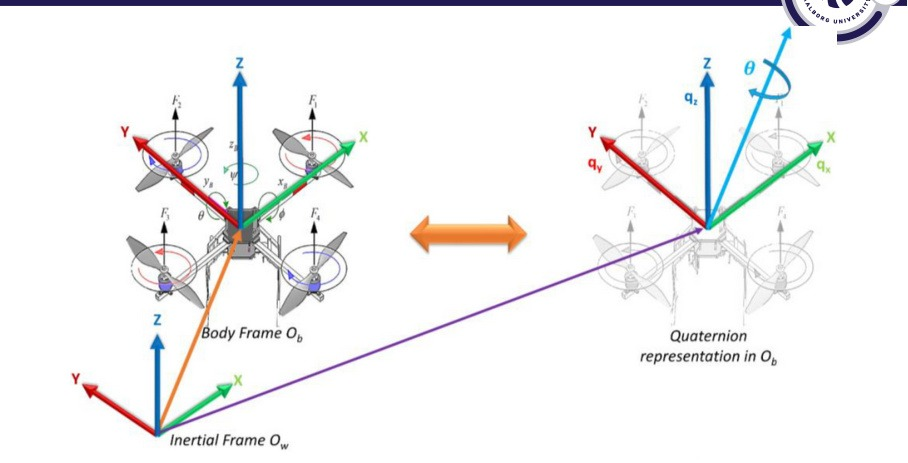
\includegraphics[width=\linewidth]{slide-31.jpg}
  \caption{Left: a drone described in the inertial frame $O_w$ and
           body frame $O_b$ using Euler-angle axes.
           Right: the same orientation described using a quaternion
           $\mathbf{q} = [q_x,\, q_y,\, q_z,\, \theta]$ in the body
           frame --- a single compact vector replaces three sequential
           rotation angles.}
  \label{fig:slide31}
\end{figure}
\todo{Maybe look at the quaternoins a bit more maybe a video will do}

\subsection*{What is a quaternion?}

A \textbf{quaternion} is a four-component number
$\mathbf{q} = [q_0,\, q_1,\, q_2,\, q_3]$ that encodes an arbitrary
3-D rotation as a single vector.
Think of it as: one component describes \emph{how much} you rotate,
and three components describe the \emph{axis} you rotate around ---
all in one compact package.

\begin{center}
\renewcommand{\arraystretch}{1.5}
\begin{tabular}{p{3.5cm} p{5cm} p{5cm}}
  \toprule
  & \textbf{Euler angles} & \textbf{Quaternions} \\
  \midrule
  Representation &
    3 angles: roll, pitch, yaw &
    4 numbers: $[q_0, q_1, q_2, q_3]$ \\
  Gimbal lock &
    Yes --- singularity at $\pm 90°$ pitch &
    No --- singularity-free for all orientations \\
  Trigonometry &
    Heavy sin/cos at every step &
    Only multiplications --- much faster \\
  Intuition &
    Easy to visualise &
    Harder to picture directly \\
  Averaging/fusion &
    Problematic (angles wrap around) &
    Clean --- average quaternions directly \\
  Used in &
    Old satellite control, simple displays &
    Spacecraft, drones, robotics, game engines \\
  \bottomrule
\end{tabular}
\end{center}

\begin{notebox}
  \textbf{Why four numbers for three rotational degrees of freedom?}\\
  A rotation in 3-D has only 3 DoF, but quaternions use 4 numbers
  subject to a constraint: $q_0^2 + q_1^2 + q_2^2 + q_3^2 = 1$
  (unit quaternion).
  The extra component is the price for avoiding the singularity.
  The constraint is maintained by \emph{normalising} the quaternion
  after each integration step.
\end{notebox}

% ==============================================================================

\section*{Slide 32 \quad Sensor Fusion: Complementary \& Madgwick Filters}

\begin{figure}[H]
  \centering
  
\includegraphics[width=\linewidth]{slide-32.jpg}
  \caption{Slide 32: properties of complementary filters (top) and
           Madgwick filters (bottom) for IMU sensor fusion.}
  \label{fig:slide32}
\end{figure}

The Kalman filter is the theoretically optimal fusion method, but it
requires matrix inversions and covariance propagation every step ---
expensive on small embedded processors.
Two lighter alternatives are widely used in practice.

\subsection*{Complementary filter}

The core idea exploits the \textbf{opposite noise profiles} of the
gyroscope and accelerometer:

\begin{itemize}[leftmargin=1.4em]
  \item \textbf{Gyroscope}: accurate and fast over short time
        (high-frequency), but bias causes slow drift over time
        (unreliable at low frequency).
  \item \textbf{Accelerometer}: noisy and sensitive to vibration
        over short time (unreliable at high frequency), but gravity
        gives a stable long-term reference for roll and pitch
        (reliable at low frequency).
\end{itemize}

The complementary filter simply applies a \textbf{high-pass filter}
to the gyro (keep the fast, short-term changes) and a
\textbf{low-pass filter} to the accelerometer (keep the slow,
long-term reference), then adds them together:
\[
  \hat{\theta} = \alpha\,(\hat{\theta}_{\text{prev}}
    + \omega\,T_s)
    + (1-\alpha)\,\theta_{\text{accel}}
\]
where $\alpha \approx 0.98$ is a tuning parameter that controls how
much you trust the gyro vs.\ the accelerometer.
Nonlinear versions are formulated on the rotation group $SO(3)$
and can handle large angles robustly while adapting to gyro bias
drift.

\subsection*{Madgwick filter}

The \textbf{Madgwick filter} is a quaternion-based alternative that
achieves near-KF accuracy at much lower computational cost:

\begin{center}
\renewcommand{\arraystretch}{1.5}
\begin{tabular}{p{4cm} p{4.5cm} p{4.5cm}}
  \toprule
  & \textbf{Kalman filter (EKF)} & \textbf{Madgwick filter} \\
  \midrule
  Representation & State vector + covariance matrix & Quaternion only \\
  Matrix inversion & Required every step & Not required \\
  Computational cost & High & Low \\
  Latency & Higher & Lower (real-time friendly) \\
  Accuracy & Optimal (if model correct) & Near-optimal in practice \\
  \bottomrule
\end{tabular}
\end{center}

Instead of propagating a covariance matrix, the Madgwick filter uses
\textbf{gradient descent} to find the quaternion orientation that
best aligns the accelerometer and magnetometer readings with gravity
and north --- a much simpler computation.

\begin{keybox}
  \textbf{Key takeaways --- Slide 32}
  \begin{itemize}[leftmargin=1.4em, topsep=2pt]
    \item Gyro: good short-term, drifts long-term.
          Accelerometer: noisy short-term, stable long-term reference.
          Complementary filter exploits this split.
    \item Madgwick: quaternion gradient descent, no matrix inversion,
          lower latency than EKF --- popular on embedded systems
          (Arduino, flight controllers).
    \item Both are alternatives to the full KF when computational
          resources are limited.
  \end{itemize}
\end{keybox}
\begin{notebox}
  \textbf{Did the 1D Kalman filter use Euler angles --- and could
  we have used quaternions instead?}\\
  The 1D Kalman filter example in Slides~23--27 used \emph{neither}
  Euler angles nor quaternions.
  It was a completely flat 1-D problem --- the states were just
  numbers (position, velocity, acceleration, bias) with no rotation
  anywhere.
  That is why a standard linear KF worked fine.\\[4pt]
  The EKF/UKF discussion was about a different, harder problem:
  \textbf{full 3-D attitude estimation}, where gyro readings are
  integrated into an orientation.
  That is where the nonlinearity comes from, and the two
  representation choices give slightly different flavours of it:
  \begin{itemize}[leftmargin=1.4em, topsep=4pt]
    \item \textbf{Euler angles + EKF}: the measurement equations
          involve $\sin\theta$ and $\cos\theta$, which are strongly
          nonlinear.
          The EKF linearises around the current estimate at every
          step.
          Near gimbal lock ($\theta \approx 90°$) the linearisation
          breaks down badly.
    \item \textbf{Quaternions + EKF (or MEKF)}: you still need a
          nonlinear filter because the measurement equations
          (matching the accelerometer reading against the rotated
          gravity vector) are still nonlinear in $\mathbf{q}$.
          But the nonlinearity is gentler --- no singularity, smoother
          functions --- so the linearisation is more reliable.
          The specialised version is called the
          \textbf{Multiplicative EKF (MEKF)}, which keeps the
          unit-quaternion constraint
          ($q_0^2+q_1^2+q_2^2+q_3^2 = 1$) intact during the update
          step.
  \end{itemize}
  Quaternions do \emph{not} eliminate the need for EKF entirely, but
  they make it work better --- no gimbal lock, more numerically
  stable.
  The Madgwick filter goes one step further and sidesteps the
  covariance matrix completely by using gradient descent instead,
  making it the lightest option of the three.
\end{notebox}

% ==============================================================================
\clearpage
\section*{Slide 33 \quad Summary}

\begin{figure}[H]
  \centering
  
\includegraphics[width=0.9\linewidth]{slide-33.jpg}
  \caption{Lecture summary: strengths and limitations of IMUs.}
  \label{fig:slide33}
\end{figure}

\begin{center}
\renewcommand{\arraystretch}{1.5}
\begin{tabular}{p{7cm} p{7cm}}
  \toprule
  \textbf{Strengths} & \textbf{Limitations} \\
  \midrule
  High sample rate (up to 1000\,Hz) &
    Inherent noise and bias cause drift \\
  Good short-term state estimation &
    Temperature and motion induce complex errors \\
  Self-contained --- no external signal needed &
    Long-term estimation requires external sensors \\
  Low cost for consumer MEMS (2--5\,EUR) &
    Performance depends heavily on calibration quality \\
  Indispensable for drone and robot navigation &
    Gimbal lock if using Euler angles \\
  \bottomrule
\end{tabular}
\end{center}

\begin{keybox}
  \textbf{The three-layer picture of an IMU system}
  \begin{itemize}[leftmargin=1.4em, topsep=2pt]
    \item \textbf{Layer 1 --- Model the errors}
          (Sections 2--3): understand every deterministic and
          stochastic error source so you know what you are dealing
          with.
    \item \textbf{Layer 2 --- Calibrate and filter}
          (Sections 4--5): remove deterministic errors via
          calibration; track stochastic bias with a Kalman,
          complementary or Madgwick filter.
    \item \textbf{Layer 3 --- Fuse with external sensors}:
          IMU provides fast, smooth short-term estimates;
          GPS/camera/barometer corrects the long-term drift.
          Together they give accurate, continuous, robust navigation.
  \end{itemize}
\end{keybox}


\end{document}

This exercise implements the 4-state Kalman filter from Slides 22--25
using the parameters
$\phi = 0.9$, $\sigma_{w_a} = \sigma_{w_b} = \sigma_\nu = 0.1$,
$b = -0.2$, $T_s = 0.001$,
and replicates the four-panel simulation figure on Slide~25.

% ─── Why only the accelerometer? ──────────────────────────────────────────────
\subsection*{Scope: accelerometer only}

\begin{notebox}
  \textbf{Why no gyroscope or magnetometer here?}\\
  A full 9-axis IMU combines three sensor types.
  For this 1-D exercise we deliberately use \textbf{only the accelerometer}.
  This strips the problem to its bare essentials: one sensor, one axis,
  four states to estimate.
  The gyroscope (angular rate) and magnetometer (heading) are essential
  for 3-D attitude estimation, but that requires the nonlinear EKF/UKF
  discussed in Section~4.
  Here we verify the linear KF structure and observe its fundamental
  limitation --- position diverges without a position sensor --- in the
  simplest possible setting.
\end{notebox}

% ─── The four states ──────────────────────────────────────────────────────────
\subsection*{The four states and why we need them}

\begin{defbox}
  \textbf{State vector:}
  $\boldsymbol{\chi}_k = \begin{bmatrix} x_k & v_k & a_k & b_k \end{bmatrix}^\top$
  \begin{itemize}[leftmargin=1.4em, topsep=4pt]
    \item $x_k$ --- position (m).
    \item $v_k$ --- velocity (m/s).
    \item $a_k$ --- true acceleration (m/s$^2$), modelled as LP-filtered noise.
    \item $b_k$ --- accelerometer bias (m/s$^2$), modelled as a random walk.
  \end{itemize}
  The accelerometer measures only $y_k = a_k + b_k + \nu_k$, so $x$ and $v$
  have \emph{no direct measurement}.
  They are estimated by integrating the acceleration estimate, but without
  a position sensor to anchor them they drift without bound --- this is
  the observability limitation shown in Slide~25.
\end{defbox}

% ─── IMU error taxonomy ───────────────────────────────────────────────────────
\subsection*{Full IMU error taxonomy --- deterministic vs.\ stochastic}

This exercise focuses on the two stochastic errors.
The table below puts them in the context of the complete error model
from Slide~16 so all error types are visible in one place.

\begin{center}
\renewcommand{\arraystretch}{1.6}
\begin{tabular}{p{1.8cm} p{3.2cm} p{2.2cm} p{6.5cm}}
  \toprule
  \textbf{Symbol} & \textbf{Name} & \textbf{Type} & \textbf{Description \& effect} \\
  \midrule
  $K_a$, $K_g$
    & Sensitivity (scale)
    & Deterministic
    & Overall gain error; corrected once during calibration. \\
  $S_a$, $S_g$
    & Scale factor distortion
    & Deterministic
    & Each axis has a slightly different gain.
      Example: the $x$-axis reads 1.02\,g when true value is 1.00\,g,
      while the $y$-axis reads 0.97\,g.
      This asymmetry causes a systematic over- or under-estimate that
      depends on the direction of motion.
      Modelled as a diagonal matrix; removed by calibration. \\
  $M_a$, $M_g$
    & Misalignment
    & Deterministic
    & The three sensor axes are not exactly 90° apart (manufacturing
      tolerance).
      Example: the $x$-axis is $0.1°$ off its ideal direction, causing
      motion along $x$ to produce a small spurious reading on $y$ and
      $z$ --- \textbf{cross-axis coupling}.
      Modelled by a skew-symmetric matrix; removed by calibration
      (specifically the \textbf{tumble test} described in Slide~28,
      where the IMU is rotated to many known orientations and the
      cross-coupling coefficients are identified). \\
  $G_g \mathbf{a}$
    & g-sensitivity (gyro only)
    & Deterministic
    & Strong linear acceleration deflects the gyroscope's proof mass
      slightly, producing a spurious rotation reading.
      Example: a racing drone pulling 5\,g at launch; the gyro output
      contains a component from the acceleration, not just rotation.
      Modelled as $G_g \mathbf{a}$; significant only in high-$g$
      manoeuvres. \\
  $T_a \Delta T$, $T_g \Delta T$
    & Temperature drift
    & Deterministic
    & Silicon spring stiffness $k$ changes with temperature, shifting
      the sensor's operating point and therefore its bias.
      Modern MEMS chips carry an on-chip thermometer and correct for this
      in real time via a factory-measured lookup table (see Slide~20).
      \begin{figure}[H]
        \centering
        
\includegraphics[width=0.5\linewidth]{slide-20.jpg}
        \caption{On-chip temperature sensing and thermal compensation
                 (Slide~20): the chip reads its own die temperature and
                 applies a stored correction curve to remove the
                 temperature-induced bias shift.}
        \label{fig:slide20ex}
      \end{figure} \\
  $\boldsymbol{\nu}_a$, $\boldsymbol{\nu}_g$
    & White noise
    & \textbf{Stochastic}
    & Fast, sample-to-sample random jitter from thermo-mechanical
      fluctuations.
      Zero mean: every sample is equally likely to be above or below
      the true value, so the average over many samples converges to
      zero --- it does not accumulate a trend.
      In the exercise: $\nu \sim \mathcal{N}(0, \sigma_\nu^2)$,
      $\sigma_\nu = 0.1$.\\
  $\boldsymbol{\epsilon}_a$, $\boldsymbol{\epsilon}_g$
    & Bias random walk
    & \textbf{Stochastic}
    & Slow, correlated drift driven by electronic \textbf{flicker noise}
      ($1/f$ noise) in the analogue readout circuitry.
      Unlike white noise, successive increments are \emph{not}
      independent --- the bias wanders continuously.
      Each increment $w_{b,k} \sim \mathcal{N}(0, \sigma_{w_b}^2)$
      is zero-mean, so the bias has no preferred direction,
      but the cumulative sum grows as $\sqrt{k}$ --- a
      \textbf{random walk}.
      This is why it cannot be calibrated away: today the bias may
      be $-0.2$\,m/s$^2$ and tomorrow $-0.25$\,m/s$^2$, with no
      deterministic pattern.
      In the exercise we model it as
      $b_{k+1} = b_k + \sigma_{w_b} \bar{w}_{b,k}$.\\
  \bottomrule
\end{tabular}
\end{center}

\begin{warnbox}
  \textbf{``Zero-mean noise does not mean zero-mean bias.''} \\
  A common confusion: the \emph{increment} $w_{b,k}$ of bias random walk
  is zero-mean (equally likely to go up or down each step).
  But the \emph{bias itself} is the sum of all past increments ---
  a random walk --- and can drift arbitrarily far from zero over time.
  It is this accumulated drift, not any single step, that degrades the
  navigation estimate if unaccounted for.\\[4pt]
  Contrast with measurement white noise $\nu_k$: it is also zero-mean
  \emph{and} stays near zero at every instant because each sample is
  independent.
  White noise affects individual readings but averages out over time;
  bias random walk corrupts the mean itself and therefore does not
  average out.
\end{warnbox}

% ─── System matrices ──────────────────────────────────────────────────────────
\subsection*{System matrices}

\[
\boldsymbol{\Phi} =
\begin{bmatrix}
  1 & T_s & 0    & 0 \\
  0 & 1   & T_s  & 0 \\
  0 & 0   & \phi & 0 \\
  0 & 0   & 0    & 1
\end{bmatrix},
\quad
Q =
\begin{bmatrix}
  0 & 0 & 0           & 0           \\
  0 & 0 & 0           & 0           \\
  0 & 0 & \sigma_{w_a}^2 & 0        \\
  0 & 0 & 0           & \sigma_{w_b}^2
\end{bmatrix},
\quad
H =
\begin{bmatrix} 0 & 0 & 1 & 1 \end{bmatrix},
\quad
R = \sigma_\nu^2
\]

With $\phi = 0.9$, $\sigma_{w_a} = \sigma_{w_b} = 0.1$, $\sigma_\nu = 0.1$,
$T_s = 0.001$.

% ─── Kalman filter equations ──────────────────────────────────────────────────
\subsection*{Filter equations (same as Slide 24)}

\textbf{Initialisation:} $\hat{\boldsymbol{\chi}}_{0|-1} = \mathbf{0}$,
$P_{0|-1} = I$.

\textbf{Step A --- Measurement update:}
\[
  \tilde{y}_{k|k-1} = y_k - H\hat{\boldsymbol{\chi}}_{k|k-1}, \qquad
  K_k = P_{k|k-1}H^\top\!\left(H P_{k|k-1}H^\top + R\right)^{-1}
\]
\[
  \hat{\boldsymbol{\chi}}_{k|k} = \hat{\boldsymbol{\chi}}_{k|k-1} + K_k \tilde{y}_{k|k-1}
\]
\[
  P_{k|k} = (I - K_k H)\,P_{k|k-1}\,(I - K_k H)^\top + K_k R K_k^\top
  \quad \text{(Joseph form)}
\]

\textbf{Step B --- Time update:}
\[
  \hat{\boldsymbol{\chi}}_{k+1|k} = \boldsymbol{\Phi}\,\hat{\boldsymbol{\chi}}_{k|k},
  \qquad
  P_{k+1|k} = \boldsymbol{\Phi}\,P_{k|k}\,\boldsymbol{\Phi}^\top + Q
\]

% ─── Results ──────────────────────────────────────────────────────────────────
\subsection*{Results --- replicated slide 25}

\begin{figure}[H]
  \centering
  
\includegraphics[width=\linewidth]{slide-25.jpg}
  \caption{Slide~25: reference result.
           Blue = true signal; Red = KF estimate.
           From top: position $x_k$, velocity $v_k$,
           acceleration $a_k$, bias $b_k$.}
  \label{fig:ex1slide25}
\end{figure}

\begin{center}
\renewcommand{\arraystretch}{1.6}
\begin{tabular}{p{2.2cm} p{6cm} p{5.5cm}}
  \toprule
  \textbf{State} & \textbf{What happens} & \textbf{Why} \\
  \midrule
  Position $x_k$ &
    True signal drifts to $\approx -20$ over 50\,s.
    KF estimate stays near 0. &
    $H = [0\ 0\ 1\ 1]$ --- position is \textbf{unobservable}.
    Without a position sensor the filter has nothing to anchor on. \\
  Velocity $v_k$ &
    Same divergence as position. &
    Velocity is also unobservable for the same reason. \\
  Acceleration $a_k$ &
    Estimate closely tracks the true random signal. &
    $a_k$ enters the measurement directly; once bias is known the
    filter can recover it. \\
  Bias $b_k$ &
    Estimate starts at 0, converges to $-0.2$ within $\approx 10$\,s. &
    Bias is also directly in the measurement ($y = a + b + \nu$).
    The KF separates $a$ and $b$ by exploiting their different dynamics
    ($a$ fluctuates fast via $\phi$; $b$ changes slowly as a random
    walk). \\
  \bottomrule
\end{tabular}
\end{center}

\begin{keybox}
  \textbf{Key takeaways --- Exercise 1}
  \begin{itemize}[leftmargin=1.4em, topsep=2pt]
    \item The KF successfully identifies the unknown bias $b = -0.2$
          from the raw accelerometer stream alone --- without ever being
          told its value.
    \item Position and velocity drift because they are \textbf{unobservable}
          with only an accelerometer.
          Adding a GPS or UWB fix would add rows to $H$ and stop the
          drift.
    \item Bias random walk is stochastic: each step is zero-mean, but the
          accumulated bias is not --- it wanders.
          The KF tracks this drift continuously.
    \item Deterministic errors (scale factor, misalignment, g-sensitivity,
          temperature) are removed by pre-calibration (tumble test).
          Only the residual stochastic errors remain for the filter to handle.
  \end{itemize}
\end{keybox}

\end{document}
